\PassOptionsToPackage{main=english}{babel}

\documentclass[thesis]{mi-document}

% custom packages and commands
\usepackage[table,xcdraw]{xcolor}
\usepackage{multirow}
%\usepackage{wrapfig}
%\usepackage{floatrow}
%\newfloatcommand{capbtabbox}{table}[][\FBwidth]

\master

\title{Acquisition of a German Fan Fiction Corpus and Analysis in the Context of Gender Representation}
\author{Jonathan Sasse}
\semester{SS 2022}
\course{Master's Thesis}
\module{[z.B. MEI-M 04 (B.A.)]}
\dozent{[Seminarleiter]}
\studid{1872869}
\studSemester{9. Semester M.Sc. Medieninformatik}
\phone{0941/133742666} % Optional
\studSubject{Medieninformatik}
\firstReviewer{Prof. Dr. Christian Wolff}
\secondReviewer{Prof. Dr. Jürgen Reischer}
\advisor{Thomas Schmidt}
\address{Am alten Schlachthof 20, 93055 Regensburg}{} % Optional
\mail{jonathan.sasse@outlook.de}
\studMail{jonathan.sasse@stud.uni-regensburg.de}
\dateHandedIn{Abgabetermin der Arbeit}
\keywords{fan fiction; corpus acquisition; corpus analysis; nlp; gender representation; online writing}

\bibliographystyle{apacite}

\begin{document}

\counterwithout{lstlisting}{chapter}  % counter for listing does not work in AtBeginDocument

\pagestyle{empty}

\maketitle

\tableofcontents % Optional
\listoffigures % Optional
\listoftables % Optional
%\lstlistoflistings % Optional

\clearpage
\doublespacing

% https://blog.wordvice.com/video-which-verb-tenses-should-i-use-in-a-research-paper/
% The abstract is written for the potentially interested reader. While writing it, keep in mind that most readers read the abstract before they read the paper (sounds obvious, but many abstracts read like the authors did not consider this). The abstract should give an impression of what the paper will be about. Do not use jargon or any abbreviations here. It should be understandable for non-specialists and even for people from fields somehow far away.

In the course of this thesis, an extensive corpus of German fan fictions was acquired.
Fan fictions are fan-made stories that use existing characters and plot elements from media such as literature, movies, or games and alter them as they see fit.
Multiple sources for this kind of stories were evaluated and the most suitable ones, \emph{FanFiktion.de} and \emph{Archive of Our Own}, were selected.
This corpus consists of 412,923 stories, their chapters and reviews, as well their respective authors and metadata.
To analyze the corpus, we used the state-of-the-art named-entity recognition model \emph{FLAIR} to extract story characters with their number of occurrences, trained an LSTM model using \emph{TensorFlow} and \emph{Keras} to predict the genders of these characters, and in the process counted all personal pronouns used.
We can confirm previous findings regarding a dominance of female authors, male character portrayals and erotic narratives across all genres.
The observed use of gender-specific personal pronouns further supports these claims.
In addition, we find that younger authors feature more female characters and write less about otherwise overrepresentative all-male relationships.


\clearpage
\pagestyle{headings} % Seitennummern und Kapitelbezeichnungen anzeigen

\chapter{Introduction}\label{ch:intro}

%Die Einleitung muss nicht zwingend kreativ oder originell sein, sondern ergibt sich aus der Arbeit. Da sich der genaue Inhalt und die Ergebnisse während der Bearbeitung ändern können, muss die Einleitung eventuell später angepasst werden. Inhaltlich grenzt die Einleitung das Thema genau ein mit Formulierungen wie „diese Arbeit beschäftigt sich mit XY“. Danach sollte aufgezeigt werden, inwiefern die Problemstellung für die Medieninformatik relevant ist, sowie die einzelnen Ziele der Arbeit. Abschließend wird der inhaltliche Aufbau der Arbeit erläutert. Allgemeinsätze wie „immer mehr Menschen verwenden Computer“ sollten unbedingt vermieden werden.

Scrolling through fan fiction archives, one can find a wide variety of stories, ranging from the most innocent to the most explicit.
Archive warnings, age restrictions, or many stories that deviate from heteronormativity have the potential to scare off readers.
For many, this is precisely the refuge where they can express their artistic abilities, their desires and inclinations in the form of stories, whether deviating from social norms or not.
But fan fiction sites are not just a platform for sharing stories, it's a vibrant fan community.

While fan fiction is a place for many to flourish, it represents a great opportunity for researchers in the area of natural language processing (NLP), digital social science and digital humanities as well.
There is no shortage of web-based, freely accessible large bodies of narrative texts with rich metadata.
For researchers, this offers the potential for large-scale analysis utilizing the wide variety of writing styles, social science observations such as the evolution of social norms in the anonymity of the Internet, or the development and evaluation of new methods~\citep{Yoder2021FanfictionNLP:Fanfiction, Liu2019DENS:Analysis, Muttenthaler2019AuthorshipN-grams, Vilares2019HarryLanguage, Zhang2019GeneratingFiction}.
Consequently, there are already many studies in that field.

While most of these focus on English-language texts and corpora, in this paper we would like to examine specifically German fan fiction.
The objective of this work is therefore to acquire a corpus of German fan fiction from suitable sources that is as comprehensive as possible.
In addition to the stories, users and reviews, this should incorporate all available metadata.
We then examine the elicited texts with regard to the representation of the characters' genders.

First, we will highlight previously conducted studies that have addressed a similar research question~\ref{ch:rw}.
Then, potential sources for fanfictional texts will be located and a suitable tool for scraping the data will be evaluated and implemented.
After the data acquisition is completed, the data is preprocessed by extracting appearing story characters and gender-specific personal pronouns with their frequencies.
For determining the gender of characters, a suitable neural network model is trained. % recurrent neural network model
Finally, the results will be presented and discussed.

The entire source code including all web crawlers, programs and scripts, as well as all figures presented in this paper and beyond, and a detailed \emph{README} can be found on \emph{GitHub}\footnote{https://github.com/Cele3x/fanfiction}.
Due to legal restrictions, the corpus is currently only available on request\footnote{jonathan.sasse@ur.de}.

%Der Hauptteil beginnt mit einem kurzen Kapitel zu den Zielen der Arbeit. Bei sehr kurzen Arbeiten, wie einer Seminararbeit, ist dieser Punkt meist mit der Einleitung schon abgedeckt. Darauf folgt der aktuelle Forschungsstand zum Thema. Dabei werden unterschiedliche Ansätze vorgestellt und ihre Vor- und Nachteile aufgezeigt. Je nach Art des Themas fallen die weiteren inhaltlichen Bestandteile unterschiedlich aus. Im Anhang A befinden sich die inhaltlichen Bausteine für eine theoretische, eine konstruktive (Paradigma der „Design Science“) oder eine empirische Arbeit (Paradigma der „Behavioral Science“).

\chapter{Objectives of this Thesis}\label{ch:thesis-overview}

Missing data for possible data analysis of fan-fictional texts for the German language in digital humanities has already been determined.

We therefore want to generate a comprehensive corpus of German fan fiction texts and accompanying metadata.
Specifically, this corpus should contain all stories as well as their chapters, reviews, associated genres, and fandoms.
It should also include the authors of stories and reviews alike, as well as their profiles.
In order to subsequently analyze a distribution of gender portrayals, some preparatory steps must first be taken.

Usually, a story consists of a collection of characters.
These must first be extracted by a suitable named-entity recognition model.
Since the name of a character as such does not tell us anything about its gender, we need to train a prediction model.
In addition to counting and predicting the character names for each story, we also want to count the number of personal pronouns that refer to a particular gender.

The information obtained in this way can then be used to study gender representation, taking into account suitable metadata.

Opportunities offered by fan fiction have already been addressed and will be explored in the following chapter based on previous research in the area.
\chapter{Previous Research in the Field of Fan Fiction}\label{ch:rw}

% Related Work intro
Fan fiction is an extraordinary resource for a huge variety of freely available texts by as many authors.
Especially in the field of natural language processing (NLP), fan fiction is a great source of material, which many publications take advantage of.


\section{History of German Fan Fiction}\label{sec:history-of-german-fan-fiction}

Since this paper's research is about German fan fiction, it is worthwhile to look at it in terms of its history.
\citet{Cuntz-Leng2015AGermany} state in their ``A Brief history of fan fiction in Germany'' that many fan activities, objects and phenomena in Germany are unique to German culture.
In the early 19th century Karl-May (1842-1912) was (and still is) one of the most widely read, translated and adapted writers~\citep{Petzel2002DasAbenteuer-Mythos}, and the closest thing to a pop-cultural phenomenon.
The growing fan base led to a growth of the German fan fiction community in general, but was abruptly halted by two world wars and the repressive politics of National Socialism.
According to \citet{Odin2008TownsIdentity}, Germans are still struggling with this trauma and loss of identity as of today.
The introduction of the internet and the success of anime and manga~\citep{Malone2010FromEconomically} are said to have been responsible for the resurgence around the year 2000 when with \emph{Animexx}\footnote{https://www.animexx.de/fanfiction/} and \emph{FanFiktion.de}\footnote{https://www.fanfiktion.de/} two fan fiction platforms were founded.
While there were relatively few stories from the genre of anime and manga on Anglo-American fan fiction platforms like \emph{FanFiction.Net}\footnote{https://www.fanfiction.net/} ($25.3\%$) and \emph{Archive of Our Own}\footnote{https://archiveofourown.org/} ($12\%$), there were significantly more on \emph{FanFiktion.de} ($29\%$) and \emph{Animexx} ($49.5\%$), which only reinforces the importance of this genre for German fan fiction culture.
\begin{table}[ht]
    \centering
    \begin{tabular}{lrr}
        \toprule
        \textbf{Fandom} & \textbf{FanFiktion.de} & \textbf{Archive Of Our Own} \\
        \midrule
        Harry Potter    & 36,877 (12.2\%)        & 69,072 (4.8\%)              \\
        Naruto          & 26,404 (8.7\%)         & 9,987 (0.7\%)               \\
        Twilight        & 13,954 (4.6\%)         & 4,397 (0.3\%)               \\
        One Piece       & 8,781 (2.9\%)          & 3,175 (0.2\%)               \\
        One Direction   & 6,308 (2.1\%)          & 33,217 (2.3\%)              \\
        Yu-Gi-Oh!       & 4,522 (1.5\%)          & 2,339 (0.16\%)              \\
        Tokio Hotel     & 4,453 (1.46\%)         & 725 (0.05\%)                \\
        Supernatural    & 3,449 (1.14\%)         & 91,848 (6.3\%)              \\
        Sherlock Holmes & 2,867 (1\%)            & 72,637 (5\%)                \\
        The Avengers    & 1,074 (0.35\%)         & 53,888 (3.7\%)              \\
        Doctor Who      & 677 (0.2\%)            & 36,896 (2.5\%)              \\
        \midrule
        Total           & 303,316                & 1,452,704                   \\
        \bottomrule
    \end{tabular}
    \caption[Top 7 fandoms on \emph{FanFiktion.de} and top 5 on \emph{Archive of Our Own}.]{Top 7 fandoms on \emph{FanFiktion.de} and top 5 on \emph{Archive of Our Own}.
    Adapted from \citet[Table~1]{Cuntz-Leng2015AGermany}.}
    \label{tab:cuntz_2015_german_english_ff_comparison}
\end{table}
Table~\ref{tab:cuntz_2015_german_english_ff_comparison} from Cuntz-Leng and Mentzinger shows that German fan fiction was much less diverse than Anglo-American was.
The \emph{Harry Potter}, \emph{Naruto} and \emph{Twilight} fandoms on FF.de accounted for a very large proportion of German fanfiction in 2015, with over 25 percent of all published stories.
Because each fan fiction community differs in its ``sets of rules, the socialization and education of their members, and the popularity of certain characters, pairings, tropes, or genres'', Cuntz-Leng and Mentzinger contend that generalizing assumptions about fan fiction communities is highly questionable.
They also assumed that German fan fiction writers and readers are more likely to migrate to English-speaking areas of fan culture with their greater variety, larger readership, and less strict youth-protection regulations.

Just as important as the historical and cultural background of fan fiction is analyzing who writes fan fiction.


\section{Analyzing the Authorship and Readership of Fan Fiction}\label{sec:analyzing-the-authorship-and-readership-of-fan-fiction}

Since this paper intends to analyze gender roles, and we assume that they are directly dependent on the author and the reader, it is of particularly high importance to find out how they define themselves.

In the media industry men are observed as the dominating gender in divisions like television shows, news coverage, social media like, like \emph{Twitter}\footnote{https://twitter.com} conversations, and text authors in general~\citep{Milli2016BeyondFanfiction, Bergstrom2012WhatsIt, Bretthauer2007AMusic, Jia2015MeasuringImages, Garcia2014GenderMedia}.
The question now arises as to whether differences can be identified in the area of fan fiction.

\citet{Duggan2020WhoAO3} provides a detailed analysis of people writing \emph{Harry Potter} fan fiction on the online fan fiction repository \emph{Archive Of Our Own} (\emph{AO3}).
Target of research were the contents of almost 2,000 story paratexts as well as their authors user profiles regarding age respectively life stage, gender, location and sexuality.
This wide-scale qualitative study is based on the assumption that fan fiction is no longer the domain of female, white, straight, middle-class, adult and Anglophone people~\citep{Busse2017ACultures, HelleksonBusse2006, Scott2013TextualScott, Lothian2007YearningSpace, Stanfill2011DoingFandom}.
This is due to the fact that fan fiction has become more mainstream~\cite[74]{Barnes2015FanfictionFiction} and more accessible to ``all fans despite their ages, financial means, ethnicities, nationalities, locations, linguistic knowledge, sexualities and genders''~\citep{Duggan2022Worlds...ofFiction}.
Duggan categorizes genders in female, male, trans, genderqueer respectively genderfluid (transgender), non-binary and genderless.
For being able to make statements regarding the text authors gender the pronouns used in story paratexts and profiles were examined (see Table~\ref{tab:duggan_2020_pronouns}).
Despite the fact that the majority of fans on AO3 did not provide any extractable demographic information in their notes, the paper comes to the conclusion that ``gender identity in the \emph{Harry Potter} fandom is much more diverse than previously acknowledged'' based on the data that could be obtained.
While Table~\ref{tab:duggan_2020_gender} shows that 50.39\% stated themselves to be females, 74.02\% preferred she/her(s) pronouns (see Table~\ref{tab:duggan_2020_pronouns}) why it can be inferred that the actually number lies somewhere between those values.
\begin{table}[ht]
    \centering
    \begin{tabular}{lrr}
        \toprule
        \textbf{Gender} & \textbf{Frequency} & \textbf{Percentage} \\
        \midrule
        Female          & 64                 & 50.39\%             \\
        Non-binary      & 27                 & 21.26\%             \\
        Male            & 17                 & 13.39\%             \\
        Transgender     & 14                 & 11.02\%             \\
        Genderless      & 5                  & 3.94\%              \\
        \bottomrule
    \end{tabular}
    \caption[Gender distribution in \emph{AO3} paratexts.]{Gender distribution in \emph{AO3} paratexts.
    Adapted from \citet[Table~1]{Duggan2020WhoAO3}.}
    \label{tab:duggan_2020_gender}
\end{table}
\begin{table}[ht]
    \centering
    \begin{tabular}{lrr}
        \toprule
        \textbf{Preferred pronoun(s)} & \textbf{Frequency} & \textbf{Percentage} \\
        \midrule
        She                           & 94                 & 74.02\%             \\
        He                            & 17                 & 13.39\%             \\
        They                          & 6                  & 4.72\%              \\
        She/They                      & 4                  & 3.15\%              \\
        She/He/They                   & 2                  & 1.57\%              \\
        ``Pronounless''               & 2                  & 1.57\%              \\
        He/They                       & 1                  & 0.79\%              \\
        She/He                        & 1                  & 0.79\%              \\
        \bottomrule
    \end{tabular}
    \caption[Preferred pronoun distribution in \emph{AO3} paratexts.]{Preferred pronoun distribution in \emph{AO3} paratexts.
    Adapted from \citet[Table~2]{Duggan2020WhoAO3}.}
    \label{tab:duggan_2020_pronouns}
\end{table}
With 36.22\% non-cis individuals like genderless, non-binary and transgender outline a much larger group than previously anticipated.
Though one should assume that heteronormativity is regarded as default and is therefore not being particularly emphasized by the authors.
Lastly only 13.39\% reported themselves to be male.
There were no distinctions made between various types of genres and fandoms and rather viewed from a more general perspective.

From this it can be deduced that female individuals make up the larger proportion of readers and authors of fan fiction compared to male individuals.
Assuming that the \emph{Harry Potter} fandom can be generalized and mapped to the entire sector of fiction.


\section{Stereotypes and Gender Bias in Fan Fiction}\label{sec:stereotypes-and-gender-bias-in-fan-fiction}
Based on the assumption that the majority of fan fiction is written by women, is it possible to draw conclusions about differences in stereotypes and gender bias?

In analyzing films, books and music lyrics, women tend to be portrayed as younger, domestic, rather emotional than rational, and with a greater focus on beauty than on their intellect~\citep{Towbin2004ImagesAnimatedFilms, Gooden2001Gender19951999}.
In comparison, men are portrayed as physically stronger and more active, more violent, more economically successful, less in control of their sexuality, and emotionally cold~\citep{Emons2010HeTelevision, Bretthauer2007AMusic, Lauzen2008ConstructingTelevision, Soulliere2006WrestlingWWE}.

% Fast et al. 2016: Shirtless and dangerous: Quantifying linguistic signals of gender bias in an online fiction writing community
In a comprehensive study on a dataset of more than 1.8 billion words from the \emph{Wattpad}\footnote{https://www.wattpad.com} writing community \citet{Fast2016ShirtlessCommunity} investigated gender bias and stereotypical questions.
High-level gender statistics provided by \emph{Wattpad} on request could not confirm \citet{Duggan2020WhoAO3}$'$s thesis regarding an overrepresentation of female authors (male/female ratio was 1.16 for 655,295 stories).
To address the question of how the gender of the characters affects the actions, they examined the verbs that referred to each character.
Both male stereotypes with common verbs like \emph{thrush}, \emph{abuse} or \emph{roar}, and female stereotypes with verbs like \emph{squeal}, \emph{giggle} or \emph{shriek} could be verified with this method.
It was noteworthy, however, that the \emph{angry man} stereotype failed to show up and verbs in this category tended to have darker connotations (like \emph{beat}, \emph{rip} or \emph{snarl}).

\begin{table}[ht]
    \centering
    \begin{tabular}{lrl}
        \toprule
        \textbf{Female} & \textbf{Odds} & \textbf{Sample verbs and adjectives (female odds)}    \\
        \midrule
        weak            & 1.73          & fragile (6.3), faint (3.2), sick (1.8), tired (1.4)   \\
        submissive      & 1.66          & helpless (3.5), shy (2.9), timid (2.8), whimper (1.7) \\
        childish        & 1.54          & squeal (11.1), naive (7.8), giggle (4.9), silly (1.7) \\
        afraid          & 1.46          & shriek (4.8), frightened (2.3), shiver (1.8)          \\
        dependent       & 1.43          & clingy (3.2), vulnerable (2.5), desperate (1.8)       \\
        hysterical      & 1.25          & bitchy (11.4), dramatic (3.2), suicidal (3.1)         \\
        domestic        & 1.16          & cook (2.3), wash (1.8), marry (1.7), clean (1.5)      \\
        emotional       & 1.04          & meanest (7.9), gush (5.1), sob (37), fiery (2.8)      \\
        angry           & 1.05          & bellow (3.1), growl (2.7), curse (1.4), snarl (1.3)   \\
        \bottomrule
    \end{tabular}
    \caption[Dominant female stereotype categories.]{Dominant female stereotype categories. Adapted from \citet[Table2]{Fast2016ShirtlessCommunity}.}
    \label{tab:fast_2016_stereotype_categories_female}
\end{table}

\begin{table}[ht]
    \centering
    \begin{tabular}{lrl}
        \toprule
        \textbf{Male} & \textbf{Odds} & \textbf{Sample verbs and adjectives (male odds)}         \\
        \midrule
        strong        & 2.02          & intense (3.1), smash (2.6), intimidating (2.1)           \\
        arrogant      & 1.30          & cocky (7.1), smirk (2.8), smug (2.6), rude (1.4)         \\
        sexual        & 1.22          & sexiest (3.1), kiss (2.4), hot (2.1), flirt (1.5)        \\
        active        & 1.17          & jog (2.5), lift (2.4), dodge (1.7), spin (1.4)           \\
        dominant      & 1.15          & rich (28), protective (2.7), royal (2.0), command (1.4)  \\
        violent       & 1.10          & abuse (4.4), hurt (2.3), beat (2.0), kill (1.5)          \\
        beautiful     & 1.06          & dreamy (8.14), attractive (4.09), cute (3.3), hot (2.14) \\
        angry         & 1.05          & bellow (3.1), growl (2.7), curse (1.4), snarl (1.3)      \\
        \bottomrule
    \end{tabular}
    \caption[Dominant male stereotype categories.]{Dominant male stereotype categories. Adapted from \citet[Table~2]{Fast2016ShirtlessCommunity}.}
    \label{tab:fast_2016_stereotype_categories_male}
\end{table}

They further investigated which adjectives were used to describe characters and categorized these as well as depicted in~\ref{tab:fast_2016_stereotype_categories_female} and~\ref{tab:fast_2016_stereotype_categories_male}.
In general, stereotypical characteristics were confirmed here as well, but a relatively large number of male characters were described with the rather feminine adjective \emph{beautiful}.
As a third hypothesis, they explored the question of how stereotypes in stories affect their user ratings.
They find that many common stereotypes, such as sexual, arrogant and violent men, have a positive impact on the ratings, while others, such as strong women or domestic men, have a negative impact (see~\ref{tab:fast_2016_stereotype_categories_ratings}).

\begin{table}[ht]
    \centering
    \begin{tabular}{lrlr}
        \toprule
        \textbf{Positive with rating} & \textbf{Coefficient} & \textbf{Negative with rating} & \textbf{Coefficient} \\
        \midrule
        sexual (male)                 & +2.03                & strong (female)               & -0.96                \\
        arrogant (male)               & +1.45                & domestic (male)               & -0.66                \\
        sexual (female)               & +1.24                & afraid (female)               & -0.66                \\
        violence (male)               & +0.92                & weak (male)                   & -0.63                \\
        active (male)                 & +0.90                & domestic (female)             & -0.57                \\
        hysterical (male)             & +0.59                & strong (male)                 & -0.51                \\
        hysterical (female)           & +0.57                & dominant (female)             & -0.44                \\
        anger (male)                  & +0.56                & emotional (female)            & -0.44                \\
        violence (female)             & +0.46                & beautiful (female)            & -0.39                \\
        childish (male)               & +0.42                & weak (female)                 & -0.34                \\
        angry (female)                & +0.20                & dependent (female)            & -0.25                \\
        emotional (male)              & +0.12                & childish (female)             & -0.21                \\
        submissive (female)           & +0.02                & active (female)               & -0.03                \\
        \bottomrule
    \end{tabular}
    \caption[Categories of stereotype with positive respectively negative effects on story ratings in a logistic regression.]{Categories of stereotype with positive respectively negative effects on story ratings in a logistic regression. Adapted from \citet[Table~4]{Fast2016ShirtlessCommunity}.}
    \label{tab:fast_2016_stereotype_categories_ratings}
\end{table}

Finally, they investigated whether female authors stereotyped men in their stories and vice versa.
To this end, they trained a logistic regression model with frequency counts of words captured by their stereotype categories as feature inputs for male and female characters.
The goal here was to predict the authors gender of a story.
However, due to stereotypical features, the author could not be specified by the model and achieved only 53\% accuracy, so the authors concluded that both men and women write indistinguishably stereotypical genders.

% TODO: transition


\section{Possibilities for Natural Language Processing}\label{sec:possibilities-for-nlp}

% Milli & Bamman 2016: Beyond Canonical Texts: A Computational Analysis of Fanfiction
One of the early works focusing on similar aspects of source of material and research topic as this paper is a proceedings paper by \citet{Milli2016BeyondFanfiction}.
In their work they analyzed the possibilities provided by fan fictional texts for NLP, computational social science and the digital humanities in general.
Large-scale literary data as well as a vibrant social network provide a huge opportunity for research in these areas.
A large fan fiction corpus as depicted in Table~\ref{tab:milli_2016_corpus_summary} was collected from \emph{FanFiction.Net} and served as study object.
%\begin{figure}
%    \begin{floatrow}
%        \ffigbox{}{
%            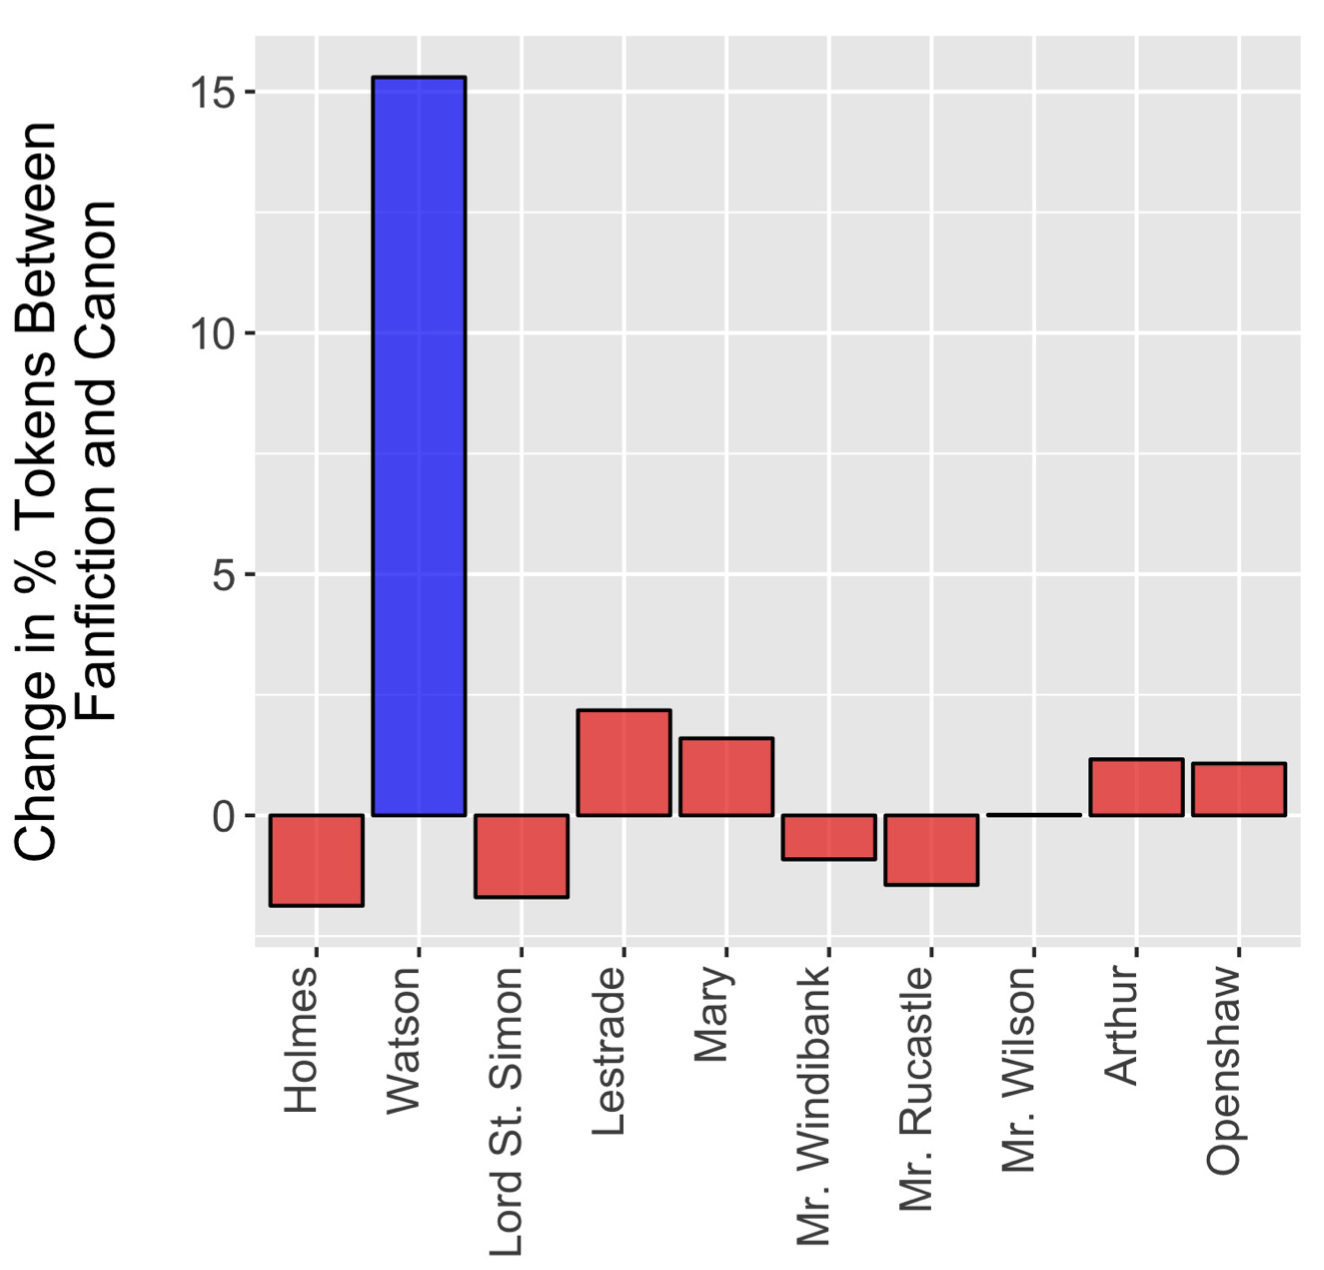
\includegraphics[width=0.5\textwidth]{figures/milli_2016_sherlock_holmes}
%            \caption[Difference in percent character mentions between fan fiction and canon for \emph{Sherlock Holmes}.]{Difference in percent character mentions between fan fiction and canon for \emph{Sherlock Holmes} \citep{Milli2016BeyondFanfiction}.}
%            \label{fig:milli_2016_sherlock_holmes2}
%        }
%        \capbtabbox{
%            \begin{tabular}{lr}
%                \toprule
%                \textbf{Type} & \textbf{Count} \\
%                \midrule
%                Canons        & 9,246          \\
%                Stories       & 5,983,038      \\
%                Tokens        & 55,264,185,653 \\
%                Reviews       & 159,914,877    \\
%                Users         & 2,093,601      \\
%                – Authors     & 1,364,729      \\
%                – Reviewers   & 1,438,721      \\
%                Languages     & 44             \\
%                \bottomrule
%            \end{tabular}
%        }{
%            \caption{A table}
%            \label{tab:table}
%        }
%    \end{floatrow}
%\end{figure}

\begin{table}[ht]
    \centering
    \begin{tabular}{lr}
        \toprule
        \textbf{Type} & \textbf{Count} \\
        \midrule
        Canons        & 9,246          \\
        Stories       & 5,983,038      \\
        Tokens        & 55,264,185,653 \\
        Reviews       & 159,914,877    \\
        Users         & 2,093,601      \\
        – Authors     & 1,364,729      \\
        – Reviewers   & 1,438,721      \\
        Languages     & 44             \\
        \bottomrule
    \end{tabular}
    \caption[Summary of the \emph{FanFiction.Net} corpus.]{Summary of the \emph{FanFiction.Net} corpus.
    Adapted from \citet[p.~2049]{Milli2016BeyondFanfiction}.}
    \label{tab:milli_2016_corpus_summary}
\end{table}
% maybe earlier in my introduction?
They stated that fan fiction with its mainly female authorship~\citep{Duggan2020WhoAO3, Barnes2015FanfictionFiction} deprioritizes the main protagonists, which are mostly male, and consists in return of more and stronger female characters~\citep{Handley2012DistressingFanfiction, Scodari2000CreatingOnline, Leow2011SubvertingFiction, Busse2009InIntroduction}.
For extracting and comparing characters they utilized the Natural Language Processing pipeline \emph{BookNLP}~\citep{Bamman2014ACharacter}.
While freely available canonical texts from \emph{Project Gutenberg}\footnote{https://www.gutenberg.org} serve as object of comparison, Milli \& Bamman can proof their hypothesis regarding deprioritization with a statistical significance of $p < 0.001$ (40.1\% female characters in canonical texts to 42.1\% in fan-written texts).
% TODO: dreprioritization of FEMALE or MAIN CHARACTERS?
\begin{figure}
    \centering
    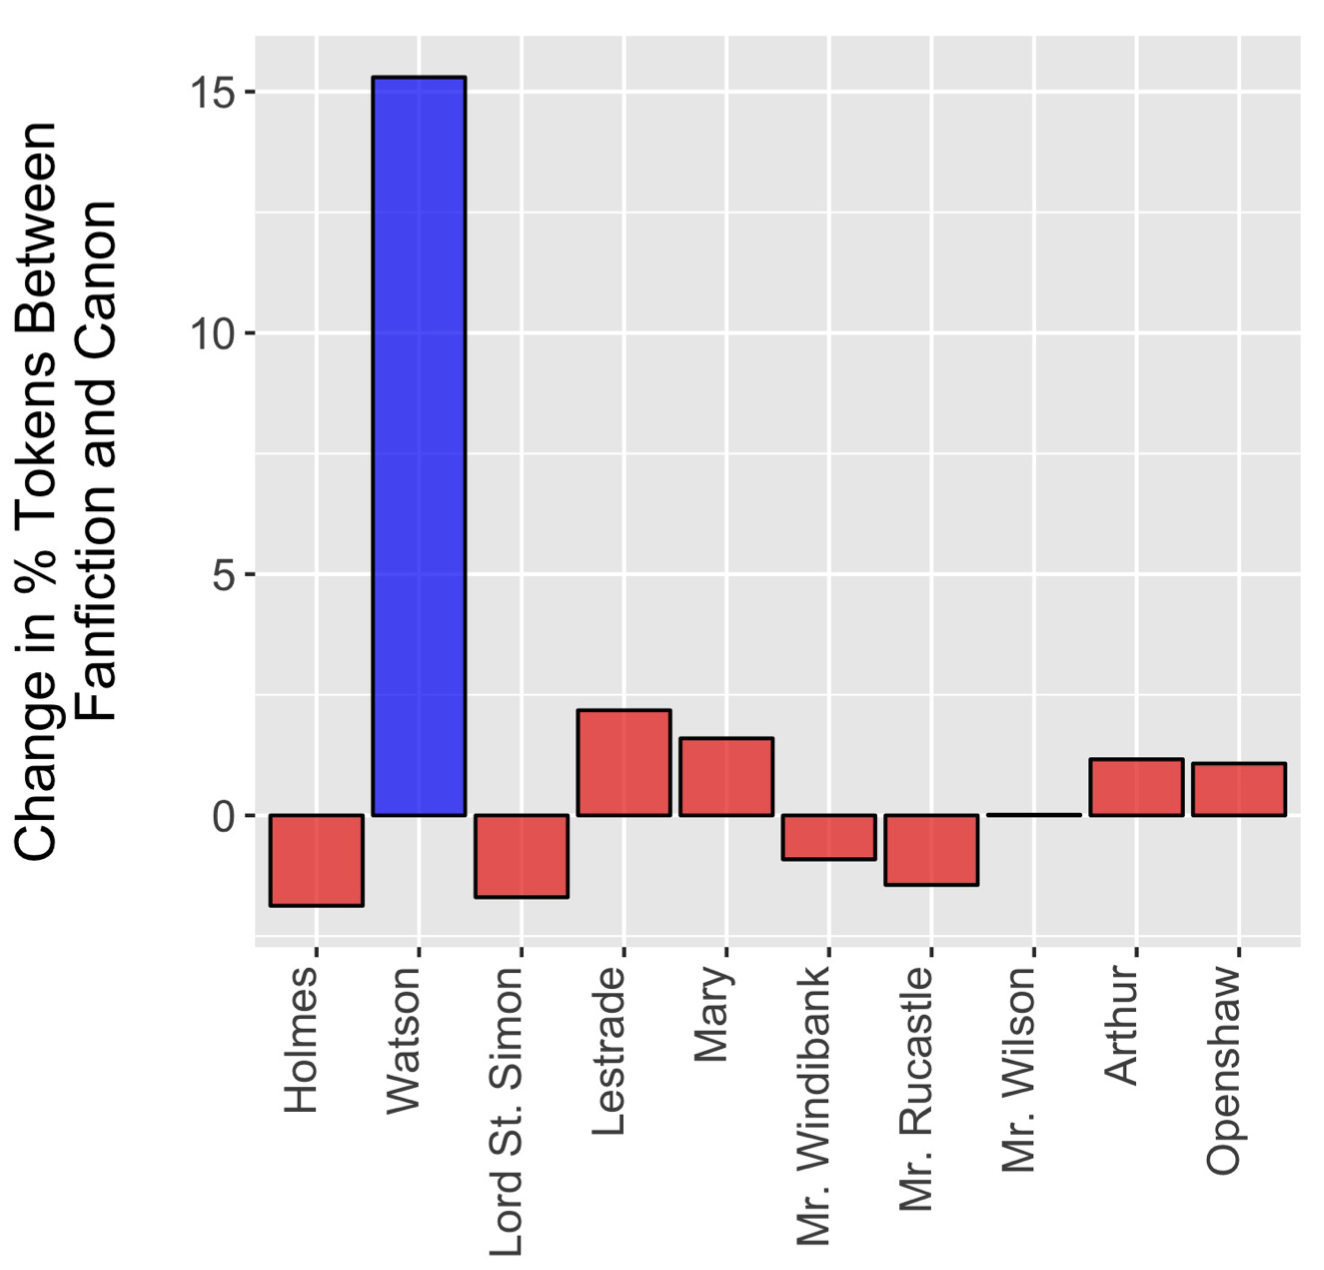
\includegraphics[width=0.5\textwidth]{figures/milli_2016_sherlock_holmes}
    \caption[Difference in percent character mentions between fan fiction and canon for \emph{Sherlock Holmes}.]{Difference in percent character mentions between fan fiction and canon for \emph{Sherlock Holmes}.
    Reprinted from~\cite[p.~2049]{Milli2016BeyondFanfiction}.}
    \label{fig:milli_2016_sherlock_holmes}
\end{figure}

As an example they presented in Figure~\ref{fig:milli_2016_sherlock_holmes} the difference of character appearances in texts about the \emph{Sherlock Holmes} fandom.
A secondary character as in \emph{Watson} receives substantially more mentions in fan fiction than in the canonical text, while the main character (\emph{Sherlock Holmes}) loses them slightly.

Furthermore, they identified that more than half of the fan-authors (52\%) are in return reviewers of other works.
In an exploratory analysis they ran a Latent Dirichlet Allocation model~\citep{Blei2003LatentAllocation} on the review texts and determined that most reviews are about positive encouragement, pleas for updates, requests to the author about the progression of the story and emotional reactions.
For training a sentiment classifier predicting the users reactions in reviews they conducted a study asking the participants to judge the sentiment towards the character expressed in the response (positive, negative, neutral or not applicable).

% Yin et al: Where No One Has Gone Before: A Meta-Dataset of the World's Largest Fanfiction Repository
% > https://dl.acm.org/doi/abs/10.1145/3025453.3025720?casa_token=BjEEdi0q0N4AAAAA:ZtJvcEJtzZy316s25giI4h1i5tR3eFGsBZQ1BxtBOMZ_ypD-WRnrwhc8fnhp0OlMP344boDG-D8W

While there are other works highlighting the possibilities that these large quantities of diversely written texts provide, they pursue other approaches that are impractical or beyond the scope of this research paper.

One of a few popular mentions is \citet{Liu2019DENS:Analysis} who fine-tuned a pre-trained BERT model for a multi-class emotion analysis using texts from previously mentioned \emph{Project Gutenberg} and \emph{Wattpad}, another platform intended for users to read and write stories.

\citet{Muttenthaler2019AuthorshipN-grams} developed and compared three n-gram models to identify authors of fan-fictional texts.
They concluded that their standard n-gram model (2 - 5 gram) performed best and a combination of different text representations best reflects the author's writing style.

The task of predicting upcoming actions from textual descriptions of scenes using \emph{Harry Potter} fan fiction was examined by \citet{Vilares2019HarryLanguage}.
A model based on an LSTM, a recurrent neural network with feedback connections, performed best for frequent actions and extensive scene descriptions, while logistic regression performed well for infrequent actions.

By collecting a million stories and their summaries on \emph{Wattpad}, \citet{Zhang2019GeneratingFiction} identified common components to describe the stories' characters.
The objective of the work was to automatically generate these character summaries using inferring salient attributes.
They developed two models of which one extracted and used attributes from the source story by ranking them, while the other classified abstractly using a list of attributes drawn from the entire corpus of stories which performed better.

\citet{Kleindienst2020InvestigatingSupernatural} took a more specific approach and studied only one fandom, the quite popular TV show \emph{Supernatural} (see also~\ref{tab:schmidt_2021_ao3_corpus}).
In doing so, they examined how the fan fiction community adapted to the source material over the time the show ran using, while using the show's scripts and 7,000 texts from the AO3 platform.
They can confirm the thesis of \citet{Milli2016BeyondFanfiction} concerning the overrepresentation of secondary characters and observed an overwhelming amount of male-male relationships in fan fiction ($91.99\%$; \citet{Tosenberger2008HomosexualityFanfiction, HelleksonBusse2006, Duggan2017RevisingFanfiction}) compared to the source material.

% etwas größer als nur 1 fandom: crossover
Not just one specific fandom, but rather the combination of individual fandoms, the so-called crossovers, were investigated by \citet{Schmidt2022AnalyzingOwn}.
They used a tool named \emph{Gephi}\footnote{https://gephi.org/} for a computational social network analysis (SNA) depicting unique character relationships visually.
They found that original characters are important for crossovers, and that popular fandoms, stories of the same genre (e.g.\ Sci-Fi) and nationality (e.g.\ British as in \emph{Sherlock Holmes} and \emph{James Bond}) are often linked.

These are just a few examples that show the possibilities offered by the analysis and study of fan-fictional texts.


\section{Analyzing German Fan Fiction}\label{sec:german-fan-fiction} % TODO: working title

Because most fan fiction gets published in the english language and though an increasing number of german authors tend to switch to it as well~\citep{Cuntz-Leng2015AGermany}, research focuses primarily on english-written texts.

% Schmidt et al. 2021: Towards the Analysis of Fan Fictions in German Language: Exploration of a Corpus from the Platform Archive of Our Own

\citet{Cuntz-Leng2015AGermany} stated in their paper about the history of german fan fiction that style, content and progression of fan fiction differ on a cultural background.
Which is why \citet{Schmidt2021TowardsOwn} gathered a corpus of 9,640 german writings from the previously mentioned \emph{AO3} platform for analysis.
While metadata and general text statistics like the most frequent words were the subject of the investigation, they identified ``attributes that are very specific and unique to German culture''.
\begin{table}[ht]
    \centering
    \begin{tabular}{lrr}
        \toprule
        \textbf{Fandom} &
        \textbf{Frequency} &
        \textbf{Percentage} \\
        \midrule
        Tatort              & 986   & 10.2\% \\
        Harry Potter        & 800   & 8.3\%  \\
        Supernatural        & 413   & 4.3\%  \\
        Sherlock (TV)       & 405   & 4.2\%  \\
        Original Work       & 349   & 3.6\%  \\
        Football RPF        & 295   & 3.1\%  \\
        Stargate Atlantis   & 220   & 2.3\%  \\
        Stargate SG         & 191   & 2.0\%  \\
        Historical RPF      & 151   & 1.6\%  \\
        Glee                & 141   & 1.5\%  \\
        \midrule
        Rest (1,603 Fandoms) & 5,830 & 58.9\% \\
        \bottomrule
    \end{tabular}
    \caption[Top 10 fandoms of the \emph{AO3} corpus.]{Top 10 fandoms of the \emph{AO3} corpus.
    Adapted from \citet[p.~4]{Schmidt2021TowardsOwn}.}
    \label{tab:schmidt_2021_ao3_corpus}
\end{table}
Next to popular fan fiction fandoms like \emph{Harry Potter} and \emph{Supernatural}, \emph{Tatort}, a german crime television show, real person fan fiction (\emph{RPF}; e.g. \emph{Football}) as well as stories about \emph{Goethe} and \emph{Schiller} (\emph{Historical RPF}) were often used as source material as seen in~\ref{tab:schmidt_2021_ao3_corpus}.
The assumption that \emph{Anime} is strongly related to the rise of fan fiction in Germany~\citep{Cuntz-Leng2015AGermany} could not be reflected in the AO3 corpus consisting only of 97 stories.
It was also noticeable that all-male romances (56\%), male characters in general (see also~\ref{sec:possibilities-for-nlp} respectively \citet{Kleindienst2020InvestigatingSupernatural}), and an excess of stories of an erotic nature dominated the corpus.
The fascination that fan fiction has with same-sex relationships has already been identified and analyzed in the humanities by \citet{HelleksonBusse2006}, \citet{Tosenberger2008HomosexualityFanfiction} and \citet{Duggan2017RevisingFanfiction}.
Furthermore, after analyzing the most frequently occurring words in the corpus, they were able to determine that they are strikingly often words that describe physical attributes.

% TODO: transition to the main part

% NOT USED:
% Hellekson & Busse: Fan Fiction and Fan Communities in the Age of the Internet: New Essays.
% > https://books.google.de/books?hl=de&lr=&id=11ODBAAAQBAJ&oi=fnd&pg=PP1&dq=Fan+Fiction+and+Fan+Communities+in+the+Age+of+the+Internet:+New+Essays.&ots=3AViPB5RG6&sig=RrWdSLLLWFStJeF7aNJQv3owuhQ#v=onepage&q=Fan%20Fiction%20and%20Fan%20Communities%20in%20the%20Age%20of%20the%20Internet%3A%20New%20Essays.&f=false
% highlight the striking dominance of slash fan fiction (stories focused on male-male romantic and erotic relationships) in the fan fiction community

\chapter{Data Acquisition}\label{ch:data-acquisition}

% multilingual
% - AO3       Cuntz-Leng2015AGermany, Duggan2020WhoAO3, Kleindienst2020InvestigatingSupernatural, Schmidt2022AnalyzingOwn
% - FF.net    Milli2016BeyondFanfiction, Vilares2019HarryLanguage
% - Wattpad   Fast2016ShirtlessCommunity, Liu2019DENS:Analysis, Zhang2019GeneratingFiction

% german
% - FF.de     Cuntz-Leng2015AGermany

In previous research multilingual archives such as \emph{Archive of Our Own}~\citep{Duggan2020WhoAO3, Cuntz-Leng2015AGermany, Kleindienst2020InvestigatingSupernatural, Schmidt2022AnalyzingOwn}, \emph{Fanfiction.net}~\citep{Milli2016BeyondFanfiction, Vilares2019HarryLanguage}, \emph{Wattpad}~\citep{Fast2016ShirtlessCommunity, Liu2019DENS:Analysis, Zhang2019GeneratingFiction} were the objects of study, while only \citet{Cuntz-Leng2015AGermany} gathered some statistical data from \emph{FanFiktion.de}, a german fan fiction website.
As can be seen, little to no research has been done in the field of German fanfiction, despite \citeauthor{Cuntz-Leng2015AGermany}$'$s~\citeyearpar{Cuntz-Leng2015AGermany} emphasis on the importance and opportunities afforded by the study of culturally diverse texts.
For this reason, we dedicated ourselves to the task of assembling and then analyzing a comprehensive corpus consisting exclusively of German fan fiction.


\section{Sources Evaluation}\label{sec:sources-evaluation}
First, we had to locate and evaluate all potential sources of fan fiction texts.
We looked at the languages provided, the number of stories (at the time of collection), the metadata provided, and whether scraping was allowed and feasible under the terms of service of each source.
Table~\ref{tab:evaluation-results} shows an excerpt of the evaluation results (see attachment for a comprehensive table).
% TODO: reference to sources table in attachments

\begin{table}[htp]
%    \renewcommand{\arraystretch}{1.5}
    \centering
%    \begin{tabular}{lllll}%{*{5}{p{15mm}}} % 5x p{15mm}
%    \begin{tabular}{*{5}{p{15mm}}} % 5x p{15mm}
%    \begin{tabular}{|l|l|l|l|l|l|} % adds a vertical spacing
    \begin{tabular}{p{3.4cm}p{2.5cm}p{2cm}p{2cm}p{2cm}} % PAGEWIDTH = 11.9
        \toprule
        \textbf{Name}                                                                                               & \textbf{Language/s} & \textbf{German Stories} & \textbf{Scraping Permitted} & \textbf{Usable} \\
        \midrule
        FanFiktion.de\footnote{https://www.fanfiktion.de/ with TOS https://www.fanfiktion.de/p/terms-of-service/0/} & German & 412.033 & Yes & Yes \\
        FanFiction.Net\footnote{https://www.fanfiction.net/ with TOS https://www.fanfiction.net/tos/} & Multilingual & N/A$^\star$ & No & No \\
        AO3\footnote{https://archiveofourown.org/ with TOS https://archiveofourown.org/tos/} & Multilingual & N/A$^\star$ & Yes & Yes \\
        wattpad\footnote{https://www.wattpad.com/ with TOS https://policies.wattpad.com/terms/} & Multilingual & 1.600 & No & No \\
        tumblr\footnote{https://www.tumblr.com/ with TOS https://www.tumblr.com/policy/en/terms-of-service/} & Multilingual & N/A$^\star$ & No & No \\
        \bottomrule
    \end{tabular}
    \caption[Results of the fan fiction source evaluation.]{Results of the fan fiction source evaluation. (${}^\star$not available; Acquisition date: January 8, 2022)}
    \label{tab:evaluation-results}
\end{table}

Sources were examined according to their provided languages, number of German stories, structure, genres, story metadata, review existence, user information and finally whether scraping is allowed due to the terms of service (TOS).
As seen in Table~\ref{tab:evaluation-results} \emph{FanFiction.NET}, \emph{wattpad} and \emph{tumblr} were excluded from the list of possible candidates for our corpus.
Although \emph{FanFiction.NET} would have been an ideal candidate for inclusion in our corpus with its substantial amount of German text (estimated only), story and user information, and structure in general, scraping in any form is prohibited.
\emph{wattpad} and \emph{Tumblr} were poorly structured, could not be filtered by language or had too few stories in German, had little to no metadata on individual stories, and again, where not allowed to scrape.
Both \emph{Archive of Our Own} and \emph{FanFiktion.de} offered a solid site structure, a large amount of German texts and rich metadata.
While \emph{FanFiktion.de} allowed scraping for non-commercial purposes, \emph{Archive of Our Own} allowed it as long as it did not interfere or disrupt with their services.

Accordingly, \emph{Archive of Our Own} and \emph{FanFiktion.de} are getting used as source material for our corpus and will be referred to as \emph{AO3} and \emph{FF.de}, respectively, in the following paragraphs.

% AO3 descibes itself as a non-commercial archive for transformative fan fiction
% AO3 texts marked as german by the author/s
% AO3: how many german texts compared to total?

Now that the sources could be determined, the next step was to decide which tool to use to obtain the data from the websites.


\section{Web Scraper}\label{sec:web-scraper}

First, the difference between the terms \emph{web crawling} and \emph{web scraping} should be clarified.
While \emph{web crawling} is about finding and discovering URLs or links from websites, \emph{web scraping} is about extracting specified data from websites~\citep{Kenny2022WebCrawling}.
Usually both procedures are needed: first to crawl the URLs of a website and second to scrape the content.

There is a wide range of tools for crawling and scraping the internet.
Factors such as customizability, scalability, the type of input data to be processed, the desired output format, the crawling interval, and the amount of data transferred in the process all play a role.
% what is the input (html)
% what is the output (database)
% what in the scraping interval (continuously)
% how much data (much)
Since we planned to scrape continuously and free of charge, Software as a Service (SaaS) platforms like \emph{ScrapingBee}\footnote{https://www.scrapingbee.com/} or \emph{Diffbot}\footnote{https://www.diffbot.com/} were not suitable.
Desktop scraper applications such as \emph{ScrapeBox}\footnote{https://www.scrapebox.com} were due to the lack of customizability impractical.
In contrast to SaaS and desktop scraper applications, frameworks like \emph{Scrapy}\footnote{https://scrapy.org/}, \emph{Beautiful Soup}\footnote{https://www.crummy.com/software/BeautifulSoup/}, \emph{pyspider}\footnote{http://docs.pyspider.org/en/latest/}, \emph{Goutte}\footnote{https://github.com/FriendsOfPhp/Goutte}, \emph{Cheerio.js}\footnote{https://cheerio.js.org/} and \emph{Puppeteer}\footnote{https://pptr.dev/} were all open source, highly adaptable and scalable, and therefore applicable to our purposes.

\subsection{Scrapy}\label{subsec:scrapy}

We have chosen \emph{Scrapy} as scraping framework because of aspects like those requirements mentioned in the previous section.
\emph{Scrapy} uses the \emph{Python}\footnote{https://www.python.org/} language, is open source, platform-independent, actively maintained, well documented, highly scalable, and got in general lots of features that solve the most common web scraping problems.
Furthermore, one can easily add extensions like proxies and fake user-agents for the obfuscation of queries, or auto-throttle capabilities for adjusting request delays based on the sites current download latency.
Auto-throttle is a particularly valuable feature for not disrupting the sites services while also being able to automatically increase the work load at low usage times, as this was for example requested by \emph{AO3} (see Section~\ref{sec:sources-evaluation}).

\begin{figure}[htp]
    \centering
    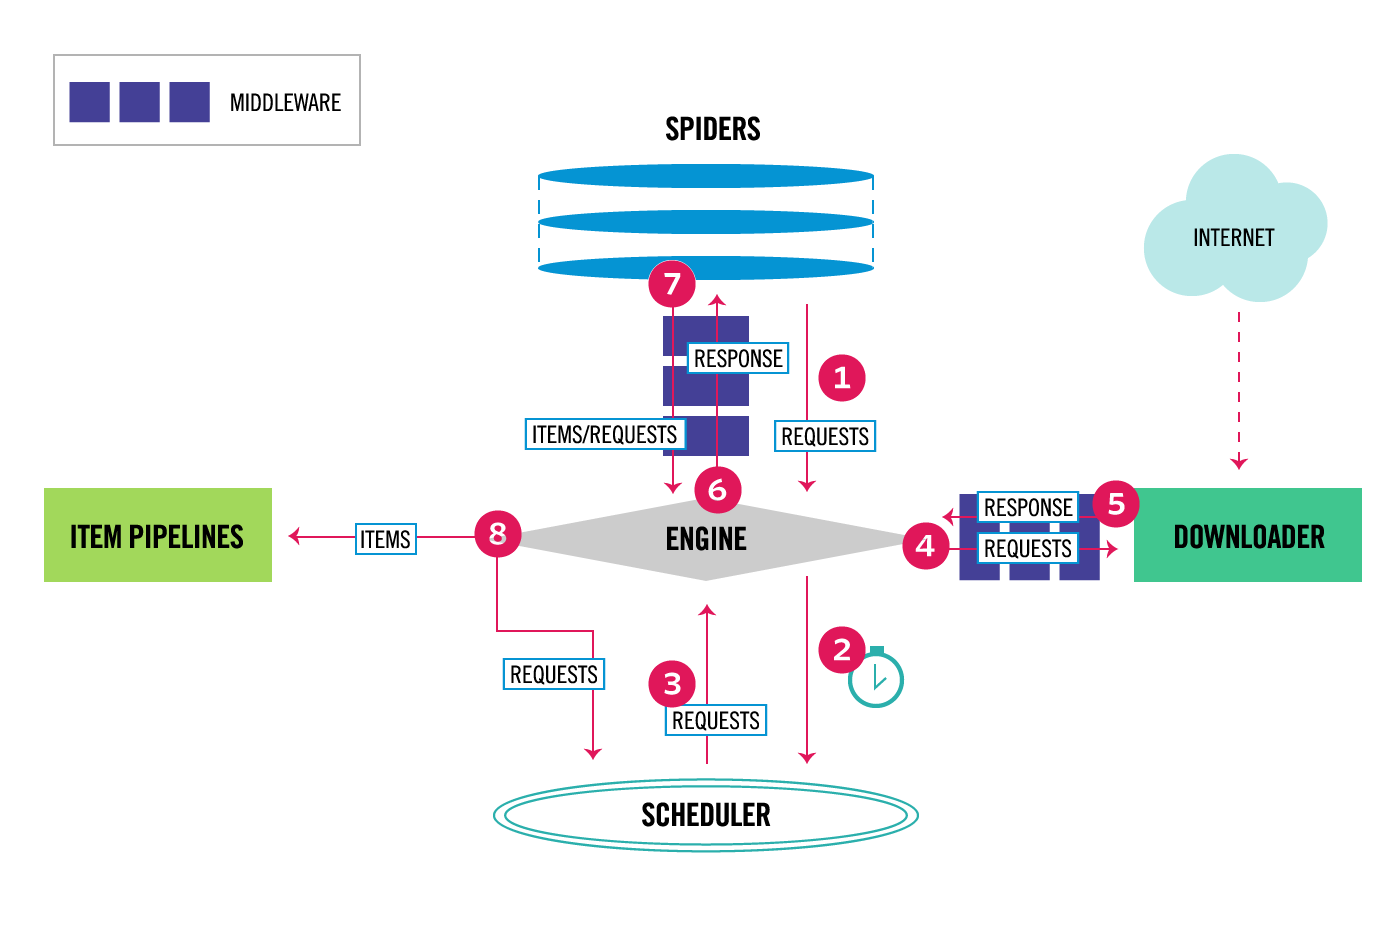
\includegraphics[width=\textwidth]{figures/scrapy_architecture}
    \caption[The architecture of the \emph{Scrapy} framework.]{The architecture of the \emph{Scrapy} framework.
    Reprinted from Architecture overview,
    In Scrapy, n.d., Retrieved October 29, 2022, from https://docs.scrapy.org/en/latest/topics/architecture.html.
    Copyright 2008–2022 by Scrapy developers.}
    \label{fig:scrapy-architecture}
\end{figure}

Figure~\ref{fig:scrapy-architecture} describes the architecture and work flow of the \emph{Scrapy} framework.
Each fan fiction archive, \emph{FF.de} and \emph{AO3}, differs in its page structure and data presentation.
It requires an individual definition of where to find the corresponding data and how to search the respective archive.
These definitions are implemented in so-called \emph{Spiders}.
The \emph{Spider} sends a request with retrieval information via the \emph{Engine} to the \emph{Scheduler}, which stores these requests and forwards them to the \emph{Downloader} with a defined delay (fixed or by using auto-throttle).
The \emph{Downloader} returns the found \emph{Items} to the \emph{Item Pipeline} if successful, where some previously programmed cleanup operations are performed and the objects are stored in a database.

The crawl process runs in a way that the \emph{Spider} seeks and follows a URL for the next page at defined positions.
To filter on a language, headers with appropriate filters must be passed to the request.

% maybe a bit more detailed

\subsection{Concurrent Crawling}\label{subsec:concurrent-crawling}

For time efficiency, we developed and ran two \emph{Spiders}, each with its own public IP, to operate on different hosts at the same time.
Each host was assigned a different fan fiction genre to crawl so that a web page did not have to be processed multiple times.
Since the database for storing the scraped data was only local, we needed a different approach for the remote host.

While the local host's \emph{Spider} stored the data directly in the database, the remote host downloaded the full HTML page, compressed it into an archive (in stacks of 1000 files), and kept a CSV list of the archive's contents.
As per previous definition in Section~\ref{sec:web-scraper}, the local host crawled and subsequently scraped the data, while the remote host merely crawled the URLs and downloaded the web page.

The CSV manifest in each archive contained a list of the names of the downloaded HTML files, the source URLs, the internal IDs of the items (stories, chapters, users or reviews;
see~\ref{subsec:db-schema}), and the chapter number (if applicable).
This list could then be used to skip URLs that had already been processed by searching for the URL found by the crawler.
The HTML files in combination with the CSV files could then be scraped by another spider without any time delay, since the data did not have to be downloaded from a website.


\section{Data Storage}\label{sec:data-storage}

Just like with the web scraper tools, we had to decide on a suitable data storage format.
We needed a storage format that would allow us to store large amounts of data in a well-structured, performant and analyzable way.
Data sets had to be easily supplemented, while avoiding duplicates and data loss.

\subsection{MongoDB}\label{subsec:mongodb}
We used \emph{MongoDB}\footnote{https://www.mongodb.com/} as database for storing the scraped data.

\emph{MongoDB} is a \emph{NoSQL}, non-relational database and has several advantages over few disadvantages for this project.
Data is stored in documents in a \emph{BSON} format which is a \emph{JSON}-like format (see Figure~\ref{fig:bson-document}).  % https://www.mongodb.com/advantages-of-mongodb

\begin{figure}[htp]
    \centering
    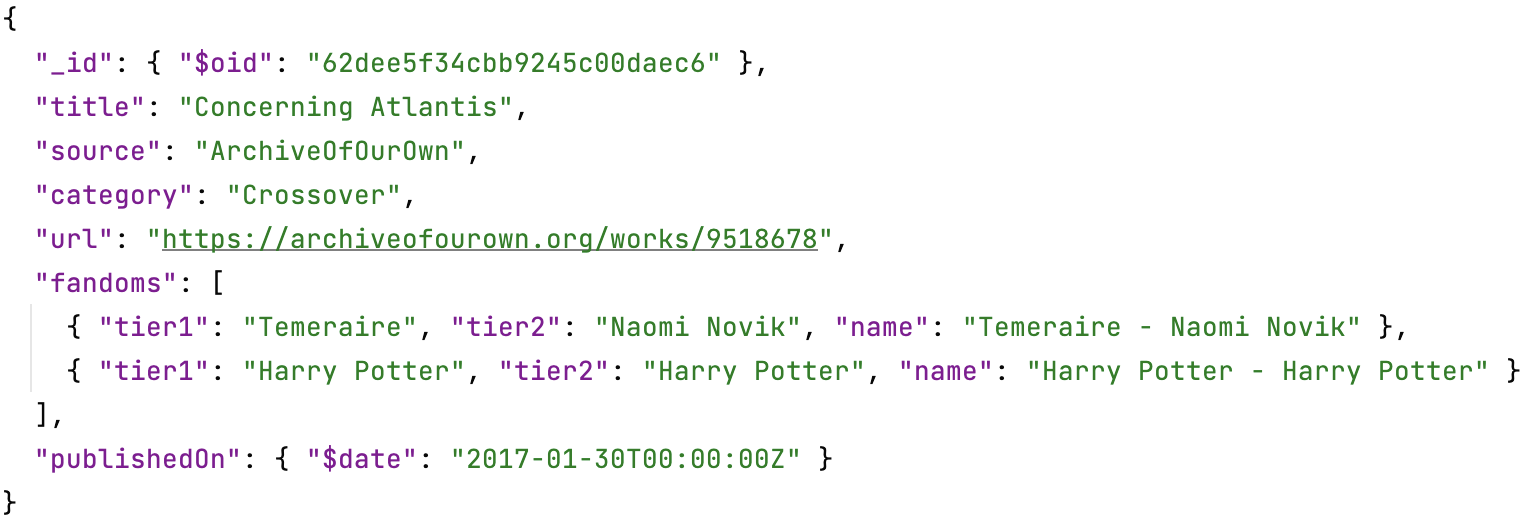
\includegraphics[width=\textwidth]{figures/bson_document}
    \caption[Excerpt of an exemplary story document in the \emph{BSON} format.]{Excerpt of an exemplary story document in the \emph{BSON} format.}
    \label{fig:bson-document}
\end{figure}

These documents are extremely flexible and can store any data without the risk of losing data because the wrong format was used~\citep{Bruce2021UnderstandingMongoDB}.
Unlike with relational database management systems (\emph{RDBMS}), which usually store the data in the 3rd normal form, \emph{NoSQL} databases generally do not use normalized forms~\citep{Chapple2022TheNormalization}.
\emph{MongoDB's} design philosophy states that data should be embedded rather than referenced, resulting in extremely efficient and performant queries since there are no expensive join queries~\citep{MongoDBAdvantagesMongoDB}.

These embeddings lead to redundancies and thus to a higher storage requirement, which is, however, negligible due to the constantly decreasing storage prices~\citep{McCallum2022HistoricalStorage}.
The schemaless structure can also cause data clutter and loss of data quality.

In addition, \emph{MongoDB} with their \emph{BSON}-documents features an easily accessible format for any programming language without the need for object-relational mappers (\emph{ORMs})~\citep{Bruce2021UnderstandingMongoDB}.
The aggregation pipeline can be utilized to build high-performance queries where data is queried and processed in multiple stages~\citep{MongoDBAggregationPipeline}.
Each stage processes its input documents and forwards them to the next stage.
For example, documents can be first filtered, then grouped, and finally sorted, with changes to the output data possible at each of these stages.

\subsection{MongoDB Schema Design}\label{subsec:db-schema}

For data acquisition, we first designed a different database schema than what was later used for the data analysis.

\minisec{Data Acquisition Schema}
Although not in compliance with the design philosophy of mongodb~\citep{MongoDBAdvantagesMongoDB}, this schema rather aligned to the principles of the 3rd normal form common in relational database models.
An excerpt of this can bee seen in Figure~\ref{fig:fan-fiction-db-acquisition-overview} while detailed database model schema can be viewed in Chapter~\ref{ch:appendices}.

% TODO: add comprensive acquisition schema to appendix

\begin{figure}[htp]
    \centering
    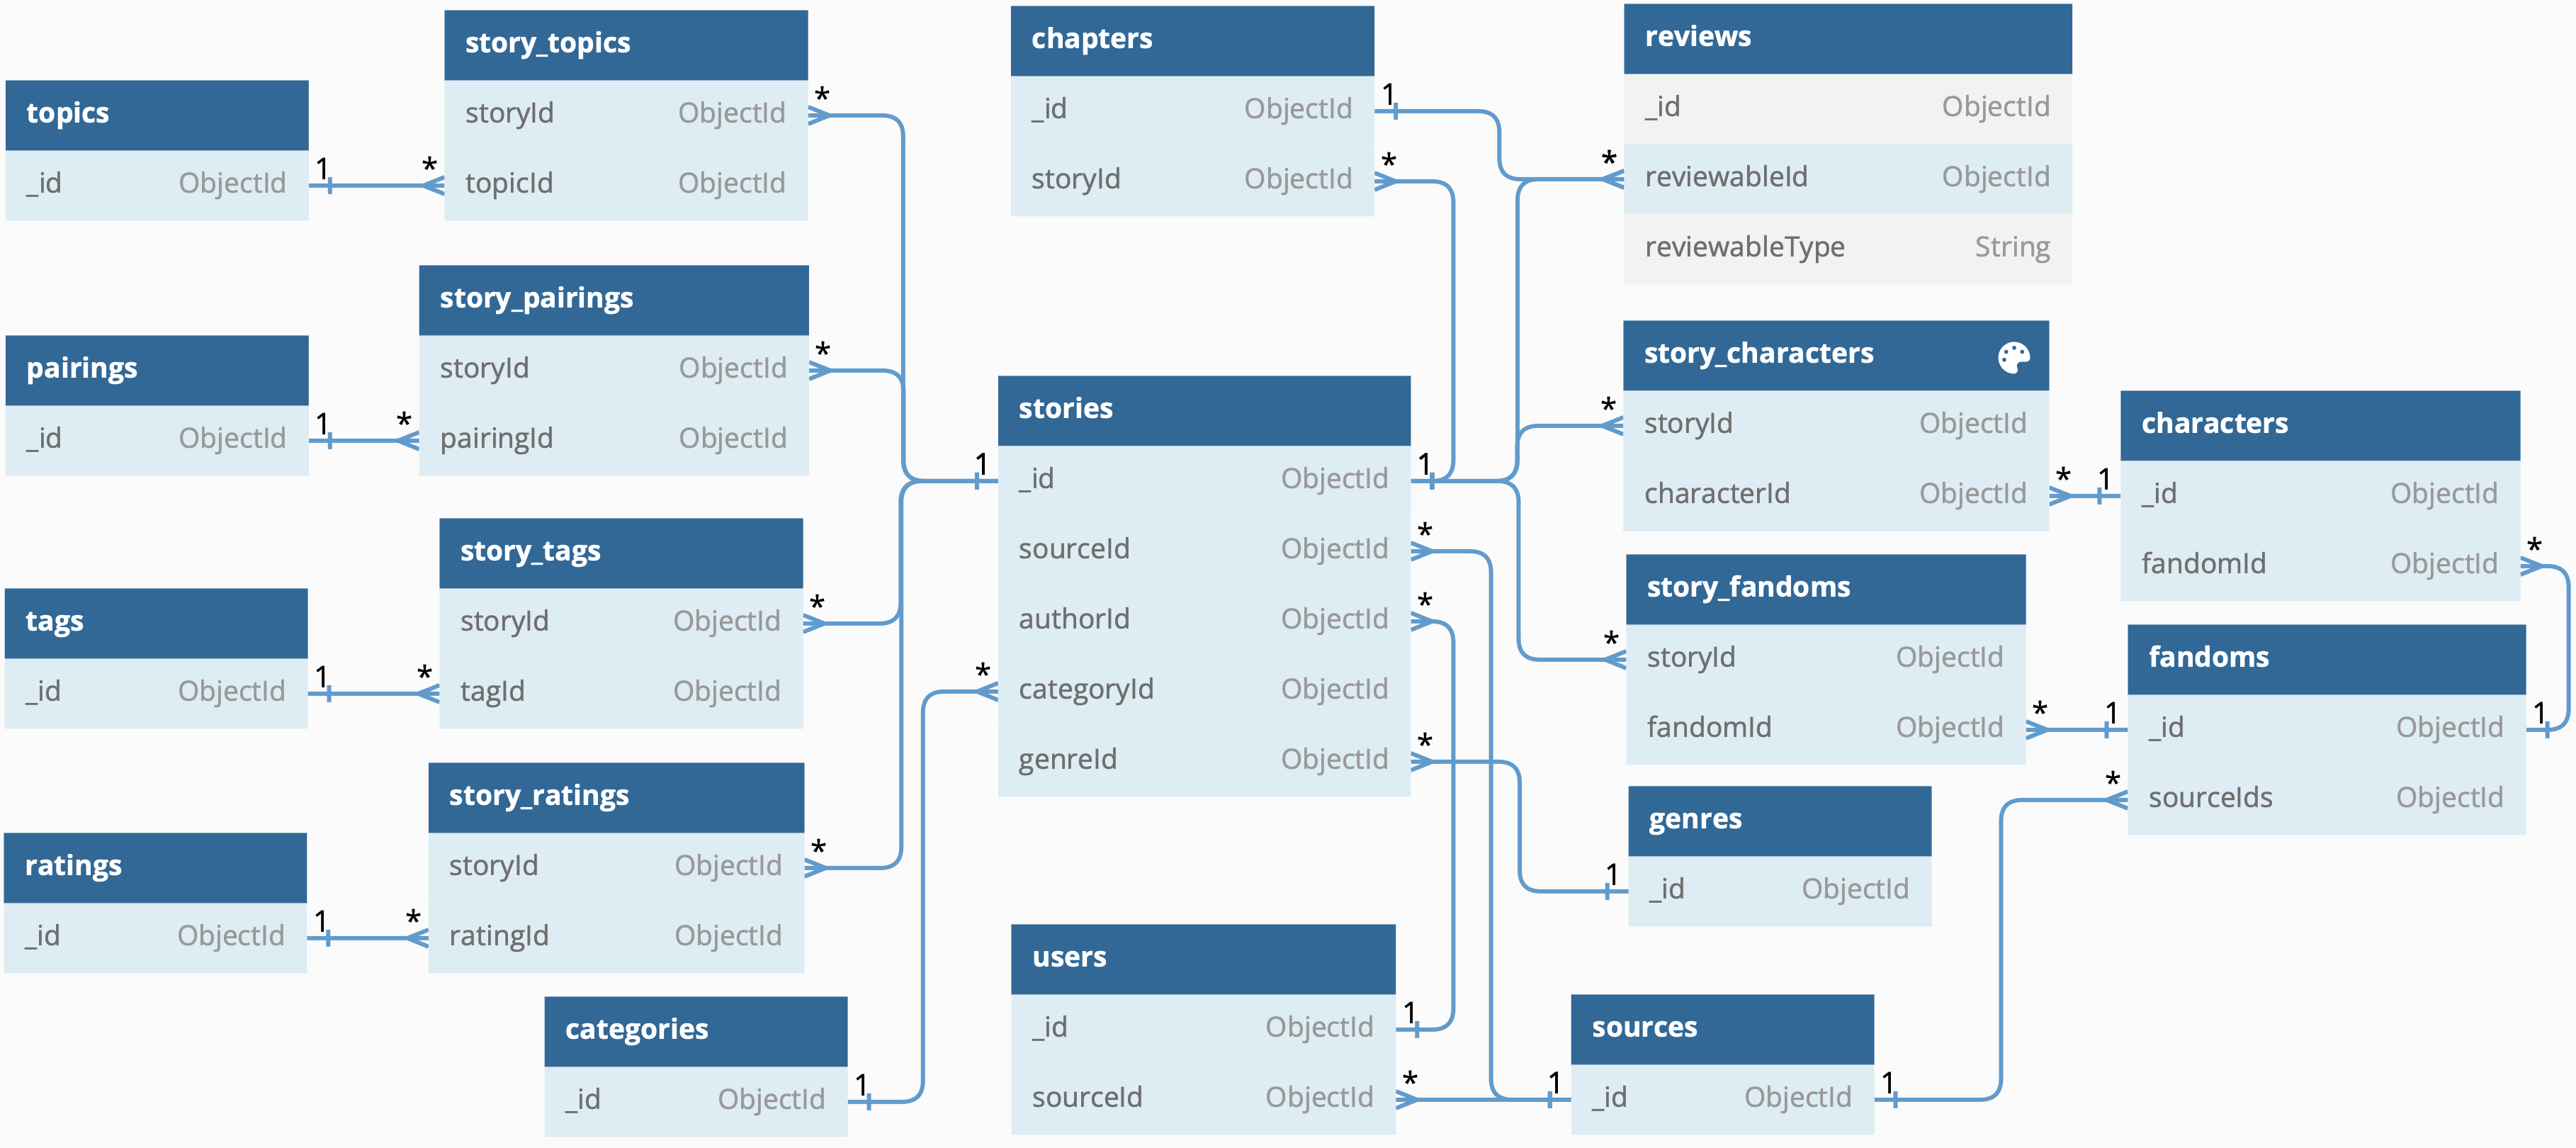
\includegraphics[width=\textwidth]{figures/fan_fiction_db_acquisition_overview}
    \caption[Excerpt of the database schema for the data acquisition.]{Excerpt of the database schema for the data acquisition.}
    \label{fig:fan-fiction-db-acquisition-overview}
\end{figure}

This relational structure had the advantage that, on the one hand, duplicates could be avoided and, on the other hand, data could be cleansed and merged more easily later.
For example, this allowed defining alternative names that are specific to each source archive.
These could be translations (e.g.~the genre could be \emph{Bücher} for \emph{FF.de} and \emph{Books \& Literature} for \emph{AO3}) or differentiating designations (e.g.~the stories pairing could be \emph{MaleSlash} for \emph{FF.de} and \emph{M/M} for \emph{AO3}).
In this way, it was possible to check during the acquisition process whether an item already existed.
Furthermore, if a fandom was to be renamed, this only had to be done in one place.
Both data quality and a consistent presentation and structure could thus be ensured.

\minisec{Data Analysis Schema}
To benefit from the capabilities of MongoDB to the full extent, we subsequently restructured the schema for analyzing the data.

Fields that were specifically needed for the scraping process were removed.
These were, for example, fields that compared the total number of chapters in the story, as indicated in the story overview, with the number of chapters already scraped, without having to query the database each time.
When a story was created in the database, an author was required.
Therefore, we initialized an empty author that contained only a user url and ID for referencing, and set a field for that user indicating that it was provisional and needed to be scraped later in the process.

All the information were then merged into four tables: \emph{stories}, \emph{chapters}, \emph{users} and \emph{reviews}.
An overview of this database schema is illustrated in Figure~\ref{fig:fan-fiction-db-analysis-comprehensive}.
%While an overview of this is illustrated in Figure~\ref{fig:fan-fiction-db-analysis-overview}, a comprehensive illustration can be found in Chapter\ref{ch:appendices}.
The chapter table contained the largest documents, since they stored the entire narrative of a story and were due to \emph{BSON}$'$s size limitation of 16 megabytes not merged into their story document.

% TODO: add comprensive analysis schema to appendix

\begin{figure}[htp]
    \centering
    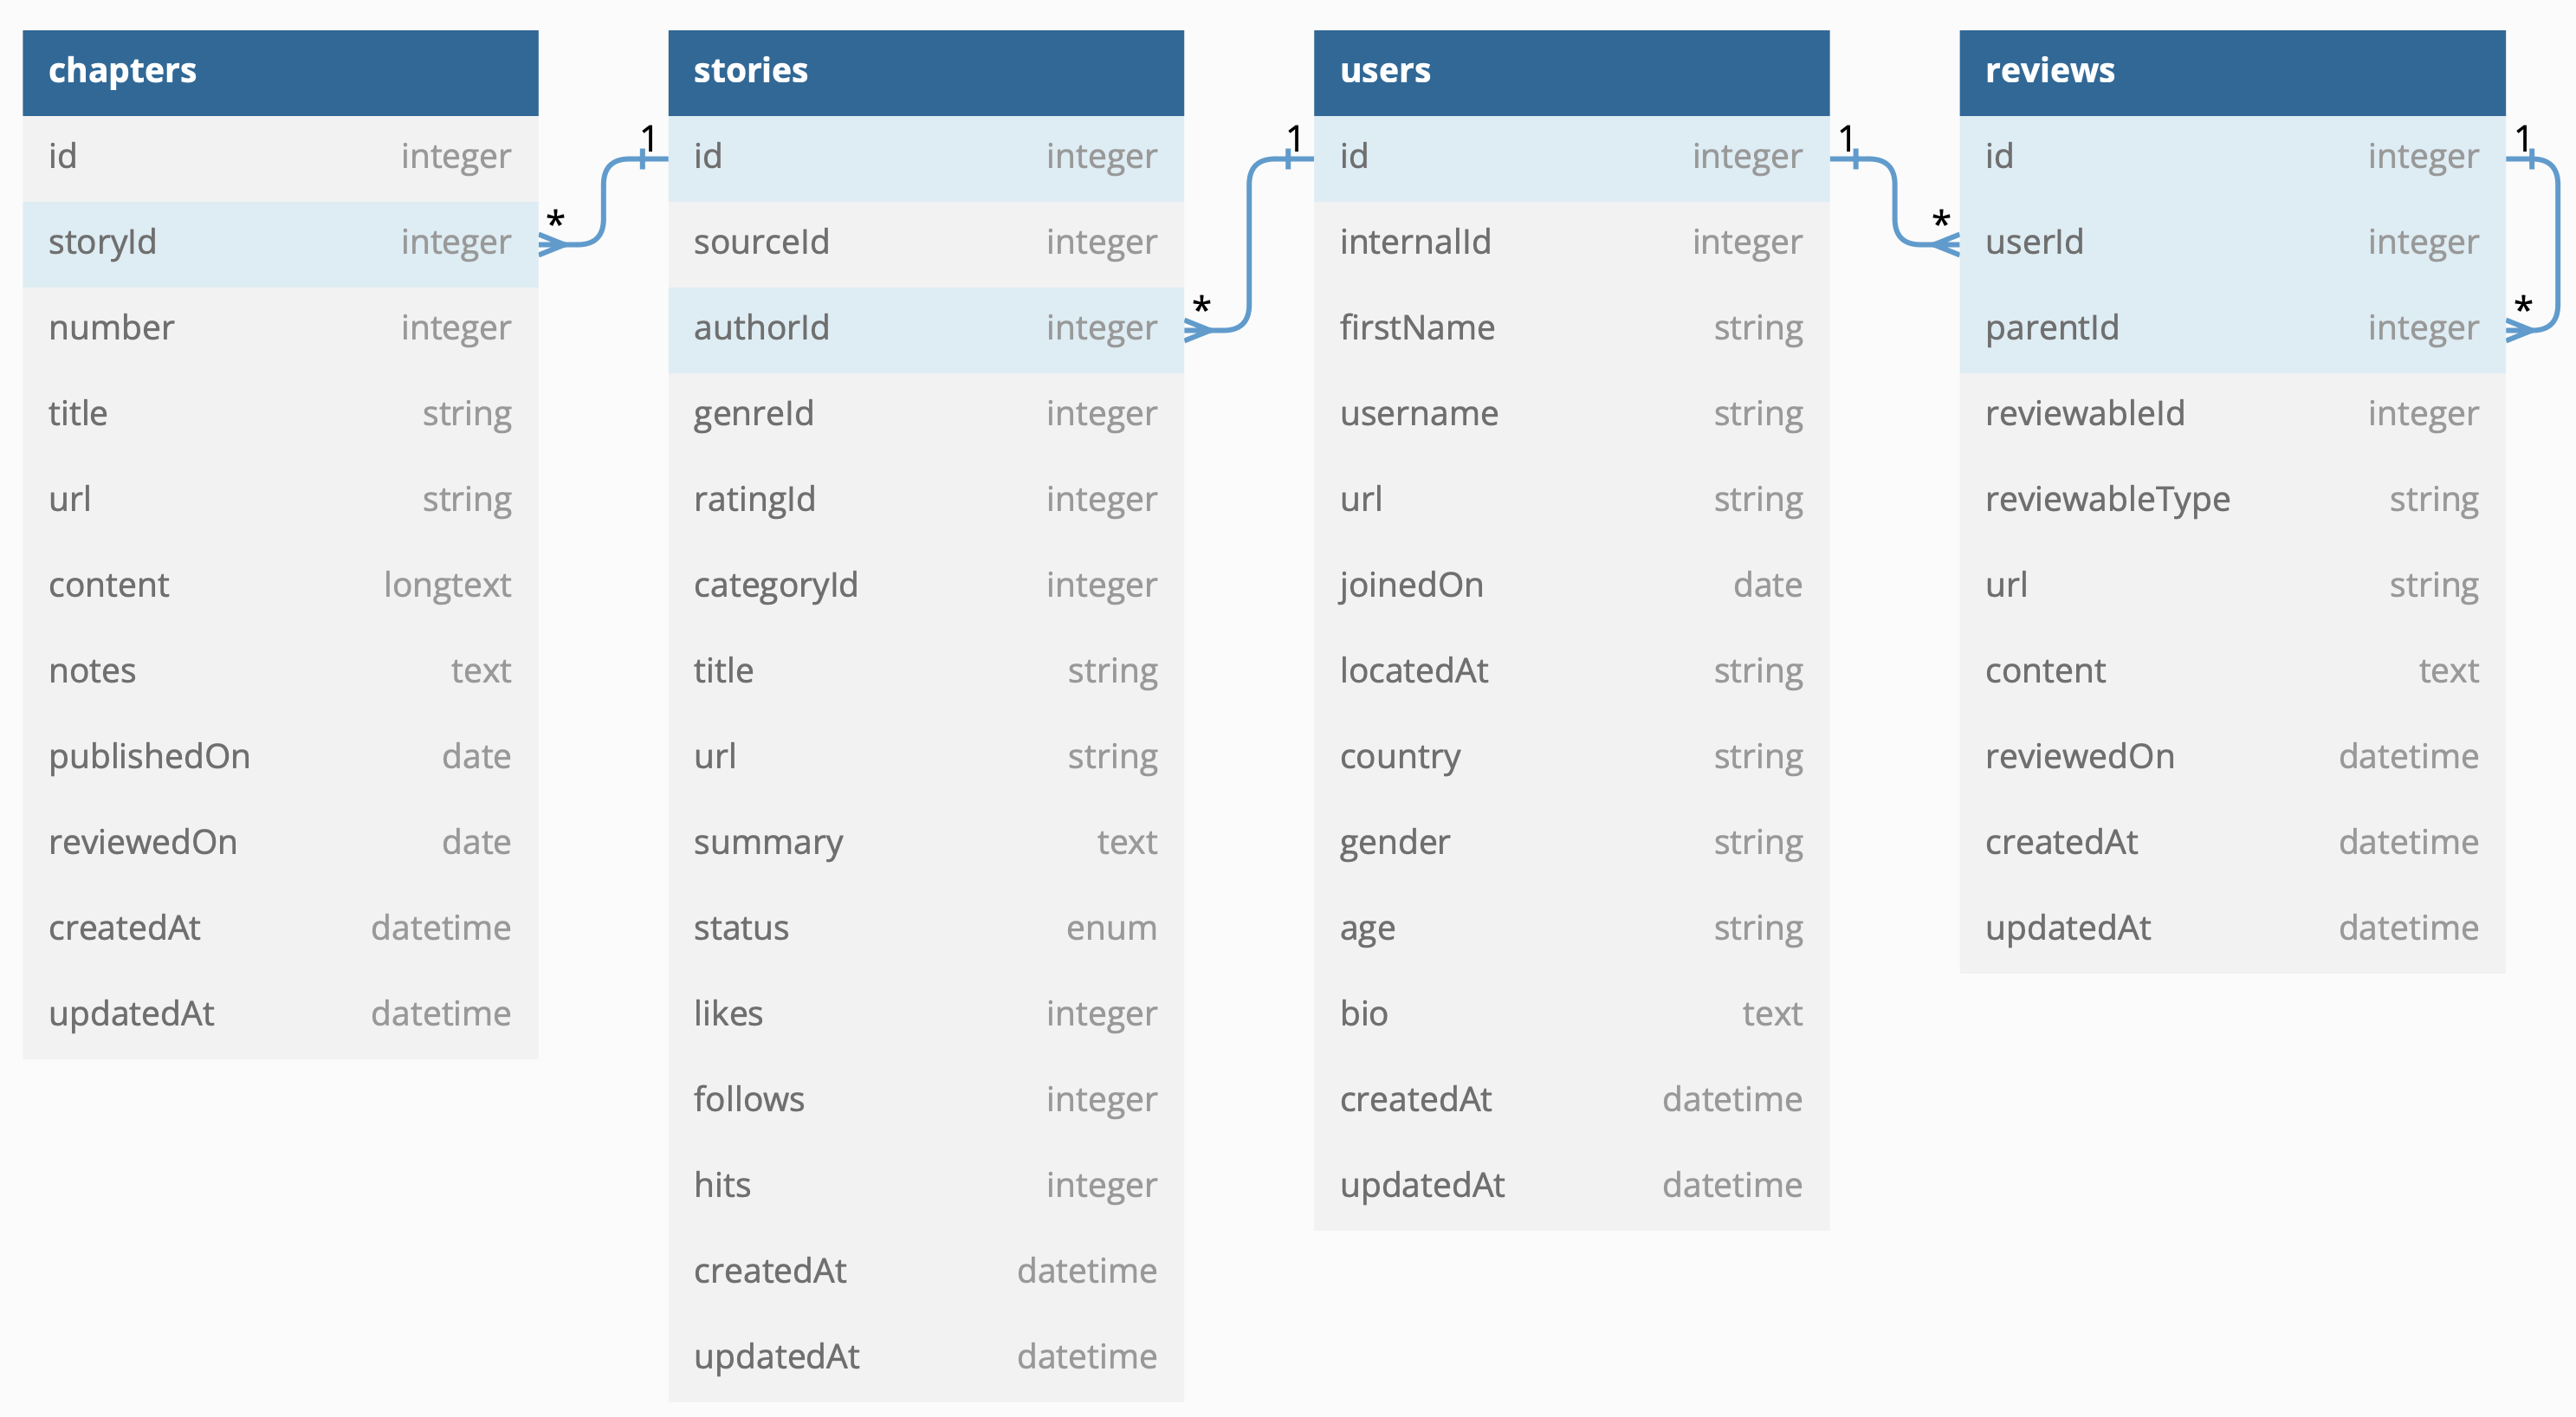
\includegraphics[width=\textwidth]{figures/fan_fiction_db_analysis_comprehensive}
    \caption[Database schema for the data analysis.]{Database schema for the data analysis.}
    \label{fig:fan-fiction-db-analysis-comprehensive}
\end{figure}

As can be seen, this schema is much leaner than the previous one.
Fields from other tables were joined into data structures such as arrays and dictionaries, disregarding the concept of avoiding duplicates.

Characters from a story were consolidated into an array containing the character name as well as the fandom the character originates from.
We structured the fandoms referenced in a story into tiers to allow easier analysis of popular fandoms with many subgenres as illustrated in Figure~\ref{fig:refactor-fandom-example}.

\begin{wrapfigure}{R}{0.65\textwidth}
    \centering
%    \textcolor{lightgray}{\frame{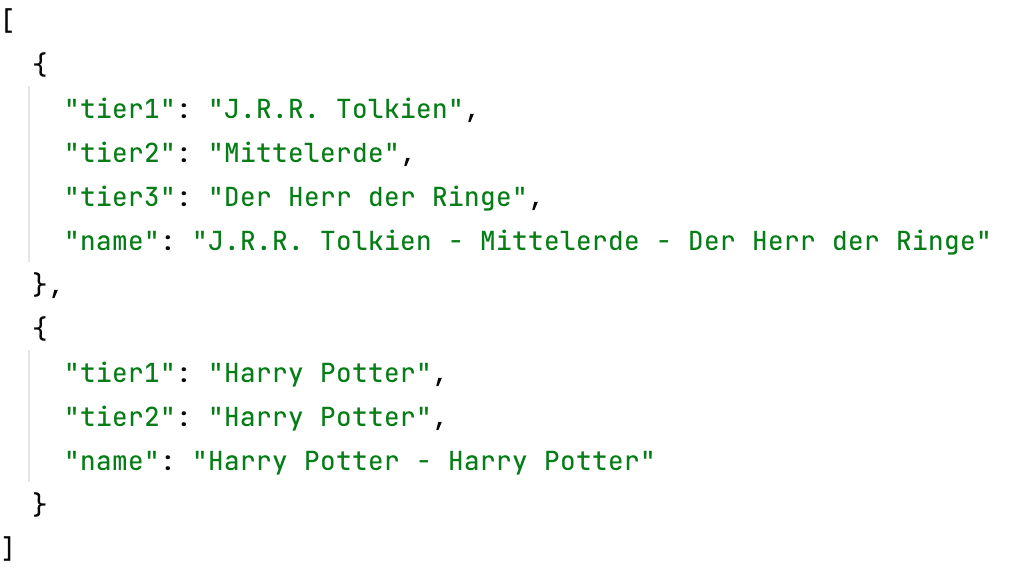
\includegraphics[width=0.4\textwidth]{figures/refactor_fandom_example}}}
    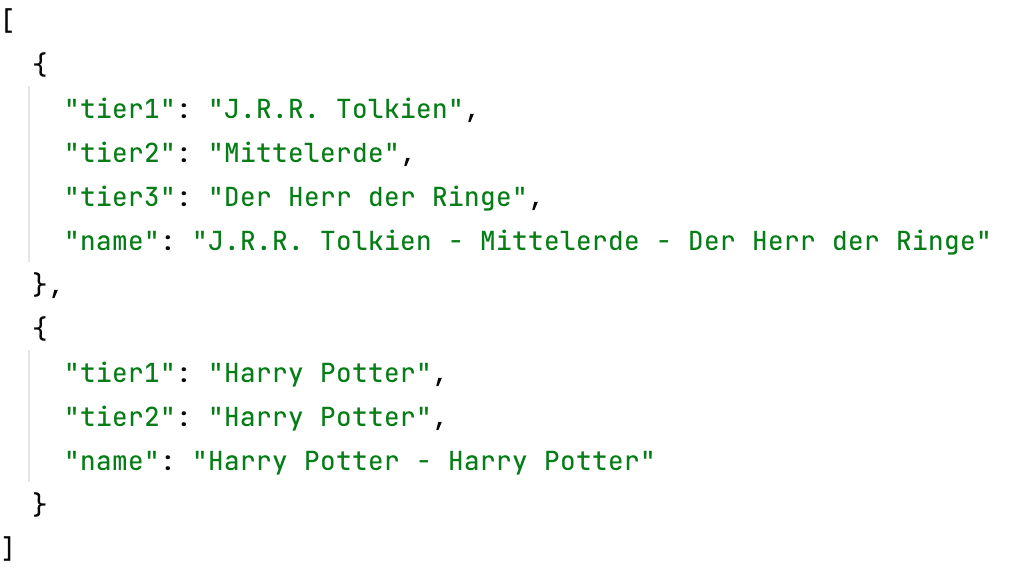
\includegraphics[width=0.6\textwidth]{figures/refactor_fandom_example}
    \caption[Example of refactored story fandoms.]{Example of refactored story fandoms.}
    \label{fig:refactor-fandom-example}
\end{wrapfigure}

\subsection{Cleansing and Plugging Data Holes}\label{subsec:cleansing-data}
In the next step of the data acquisition phase we had to fill in missing data.
This was done by implementing another set of \emph{Spiders}, one for the \emph{AO3} archive and one for the \emph{FF.de} archive.
These \emph{Spiders} were used for data that was missing from the initial scraping process by querying the database for stories and chapters that contained no content or missed other crucial elements like fandom or genre and then scraping it from the archive's website.
After scraping the missing information we still had some stories that contained no text which is why we implemented another, very simple scraper using the \emph{BeautifulSoup} library.
For that we used the URLs referencing the stories from the database and stored the obtained texts.

Numerous stories are published that contain merely an image (e.g.~a cartoon), an embedded video or audio player, a link to a story on another platform or a link to a \emph{YouTube}\footnote{https://www.youtube.com/} video.
Story chapters containing those or did not reach a specified character threshold of 15 characters were removed from the database.
Additionally, low character chapters were manually checked for their content since sometimes rather short but totally valid phrases like ``nicht schwanger'' (german for ``not pregnant'') were used while others were just placeholders.
Stories that subsequently did not include any chapters were also removed from the database.

To improve the quality of the data and increase analyzability, we have consolidated fandoms from both archives under a common name.
For the comparison of fandom names, any punctuation, whitespaces, tabs, line breaks or carriage returns were temporarily removed.
We then used the Levenshtein distance~\citep{Levenshtein1966BinaryReversals}, a metric that measures the difference between two strings based on the minimum number of single character edits such as insertions, deletions or substitutions, to determine the best match from the other archive.
For overview and manual correction, all fandoms of \emph{AO3} were then listed in a table and the most likely counterpart for each based on previous calculations was suggested.
Finally, these values were used for the consolidation in the database.

\section{Difficulties during Data Acquisition}\label{sec:difficulties-acquisition}
We had several problems when collecting the data.

The first problem was that the number of requests per minute to the archives was limited, and we needed to probe the sites for the least time delay between requests possible without being blocked by the host.
Because of the time delay and the huge amount of data available, the scraping process took its time.
To improve this, we ran a second web crawler on another machine, as described earlier in Subsection~\ref{subsec:concurrent-crawling}.
While this reduced the overall time required for scraping, it created another problem in that the fanfiction data was stored in a local database and access from this second computer was therefore not possible, so we used the CSV file as a temporary storage.

Another issue was the age restrictions for certain stories.
While this was handled at \emph{AO3} by confirming the age of majority in a popup window, at \emph{FF.de} we had to either restrict scraping of restricted stories to between 11pm and 4am, or prove our user's age with a valid ID\@.
This could be handled after authentication via \emph{Scrapy}$'$s cookie middleware, where we attached our user's session to the requests.
Sessions, on the other hand, expired after a certain time, and the stories had to be marked as age-restricted for later scraping.

\emph{AO3} distinguishes between fandoms from different media (e.g.~\emph{Sherlock Holmes \textbf{TV}} and \emph{Sherlock Holmes \textbf{Books}}), while \emph{FF.de} is much stricter in this regard and only allows one type of media (e.g.~just \emph{Sherlock Holmes}).
Consolidating the fandoms as outlined in the previous Subsection~\ref{subsec:cleansing-data} solved this issue.

Another difficulty arose from the unreliability of the users.
For example, sometimes authors used the title input box to enter the text of the story, which resulted in documents having empty chapters and overfilled titles.
These stories then had to be scraped anew after they were identified.

% AO3: non-commercial archive for transformative fanfiction
% filtered texts with links, images and (almost) empty
% Due to legal issues the corpus is currently only available upon request via e-mail (thomas.schmidt@ur.de). Reference github?
\chapter{Data Supplements}\label{ch:data-supplements}

For an improved analyzability of the data we had to append additional information to our documents.
This already covered the first steps of analysis at document level.


\section{Counting Text Tokens}\label{sec:counting-text-tokens}

First, we implemented an asynchronous script that traversed through the corpus and collected general text statistics for both chapters and stories in batches.
This included the number of sentences, words, letters and text characters.

For sentence segmentation we used the open-source library \emph{spaCy}\footnote{https://spacy.io/}, written in \emph{Python}.
It provides several pre-trained natural language models for a number of different languages, including German.
Besides its speed and ease of use, no recognition failures were detected for the sentences we tested.

After these more general supplements for the statistical analysis, we required additional information for analyzing the gender representation in the corpus.


\section{Pronouns Detection}\label{sec:pronouns-detection}

More and easier-to-analyze information was needed to verify gender distribution.
Utilizing the \emph{spaCy} library again, we implemented a script that detected all pronouns in the corpus and counted their occurrences.
This was based on the approach of~\cite{Duggan2020WhoAO3}, who analyzed pronouns in story paratexts and user profiles (see Section~\ref{sec:analyzing-the-authorship-and-readership-of-fan-fiction}).
We restricted ourselves to the personal pronouns in the third person singular, since other forms as well as the plural do not allow a clear assignment to one gender.
Consequently, these were \emph{er}, \emph{sie}, \emph{ihn}, \emph{ihm}, \emph{ihr}, \emph{seiner} and \emph{ihrer}.


\section{Extracting Story Character Names}\label{sec:ner-token-classification}

Another very time-consuming step was the filtering of all person names from the corpus on a chapter-by-chapter basis.
For this purpose, a named entity recognition (NER) model was used, which was already pre-trained for the German language and did not require any further adaptations.
We initially tested this with the fast \emph{spaCy} library, but then decided to use the state-of-the-art \emph{FLAIR}~\citep{Akbik2019FLAIR:NLP} natural language processing (NLP) framework instead for much better results.
While \citet{Milli2016BeyondFanfiction} used the \emph{BookNLP}\citep{Bamman2014ACharacter} library for this task, we were unable to utilize it, even though it was more tailored to our problem, as it was only available for the English language.
\emph{FLAIR} was trained on the \emph{CoNLL-2003}~\citep{TjongKimSang2003IntroductionRecognition} dataset, which consists of news articles from \emph{Reuters}\footnote{https://www.reuters.com/} and \emph{Frankfurter Rundschau}\footnote{https://www.fr.de/}.
The NER models provided by \emph{FLAIR} detect named entities such as persons, locations, organizations, and miscellaneous.
For this study, we limited the model to the recognition of persons, in our case characters, who appear in the stories.
Although we did not use the \emph{spaCy} library for entity recognition, we still used its previously tested sentence segmentation capabilities.
We processed each chapter at the sentence level and then appended the found person tags with the number of their appearances to the respective database document.

When using the \emph{FLAIR} models, processing was associated with accurate results, but very slow.
We have therefore tried and implemented several approaches to speed up the process.

Initially, we used the model \emph{ner-german-large}, but then decided to use model \emph{ner-multi-fast} because it was noticeably faster.
Even though it was trained on English, German, Dutch and Spanish language corpora, one could also pass German as a parameter to the sentence tagger and got equally good results.
For comparison: the German tagger (\emph{ner-german-large}) required about 1 minute and 52 seconds for a text with a length of 752 sentences (the average text length of a chapter), while the multi-language tagger \emph{ner-multi-fast} required about 1 minute and 44 seconds.
While the difference of about 8 seconds may not seem like much, it makes a significant difference in a corpora of almost two million chapters like this one.

Another approach was to use the fast \emph{spaCy} library and cleansing the results of any unwanted tokens afterwards, but this was not applicable for usable results.

For counting text tokens (see Section~\ref{sec:counting-text-tokens}), we used the concept of asynchronous batch processing for acceleration.
We tested this with various process counts and batch sizes, but the processing times increased instead of decreasing.
The likely reason was the amount of memory necessary to run multiple taggers simultaneously.

Due to one machines limitation to memory and CPU, we set up a cluster of 18 cloud computing machines to process the data in parallel.
Cloud computing space using the free quota provided by \emph{Microsoft Azure}\footnote{https://azure.microsoft.com/}, \emph{Digital Ocean}\footnote{https://www.digitalocean.com/} and \emph{Vultr}\footnote{https://www.vultr.com/} was used for this purpose.
We also configured an Ubuntu 20.04 LTS server and paired it with a static hostname for remote access so that any of these machines can access the shared database.
Each of these computers ran a single token classifier.

Due to time constraints we reduced the number of stories to be tagged to 280.000.
This was roughly equivalent to 68\% of the total number of stories.
Stories were randomly selected, locked and processed.

% session timed out for long text passages (entangled)


\section{Determine Story Character Name Genders}\label{sec:determine-character-name-genders}

After the names of the characters were extracted from the stories, the gender of each individual had to be determined.
Along with all the other code, the script for training the gender classifier can be found on \emph{GitHub}\footnote{https://github.com/Cele3x/fanfiction/}.

\minisec{Acquiring a Training Dataset}

The first step was to acquire a training dataset.
In addition to the \emph{NLTK} name corpus~\citep{StevenBird2009NaturalPython}, we obtained a large dataset from \emph{Google BigQuery}\footnote{https://cloud.google.com/bigquery/public-data} containing all names from applications for \emph{Social Security} cards for births in the \emph{United States} after 1879 provided by the \emph{United States Social Security Administration}\footnote{https://catalog.data.gov/dataset/baby-names-from-social-security-card-applications-national-data}.

To increase diversity, we have also included names from the \emph{babynames.com}\footnote{https://babynames.com/} website in our dataset.
For example, names for categories such as biblical names or names of fictional characters with corresponding gender information are listed there, but also names of various geographic origins.
The \emph{babynames.com} website names were hosted on a dynamic website, so we had to scrape them with \emph{Selenium}.
\emph{Selenium} is usually used to automate web browser interactions for testing purposes, though we used it to scrape the website and store the names in a file.

All datasets were then merged, removing all duplicates, gender-neutral names, and names that were not clearly assigned to a gender.
The result was a list of 106,000 rows, each consisting of the name and a gender classifier.

\minisec{Preprocessing the Data}

Names had to be encoded in \emph{ASCII} format because the \emph{scikit-learn}\footnote{https://scikit-learn.org/} library only accepts \emph{ASCII} characters, therefore we used the \emph{unidecode}\footnote{https://github.com/takluyver/Unidecode/} library to convert all names (e.g.~á became a).
This entailed a further duplicate check and subsequent cleanup.

Furthermore, we padded all names with spaces and converted them to lowercase.
To be able to use the data in a neural network, we also encoded the story characters in numbers.
The gender for the training set was one-hot encoded as 0 for `F' (female) and 1 for `M' (male).

\minisec{Training the Model}

For training the model we use the \emph{Keras}\footnote{https://keras.io/} library with the \emph{TensorFlow}\footnote{https://www.tensorflow.org/} backend.
The model consists of three layers: an embedding layer, a bidirectional LSTM layer and a dense layer.
We then trained the model using the Adam optimizer and the binary cross-entropy loss function.
Splitting the data into a usual training and test set size of 80\% and 20\%, respectively, we trained for 50 epochs with a batch size of 64.
For not overfitting the model, we used early stopping with a patience of 5.

\begin{figure}[htp]
    \centering
    \begin{minipage}[c]{.49\textwidth}
        \centering
        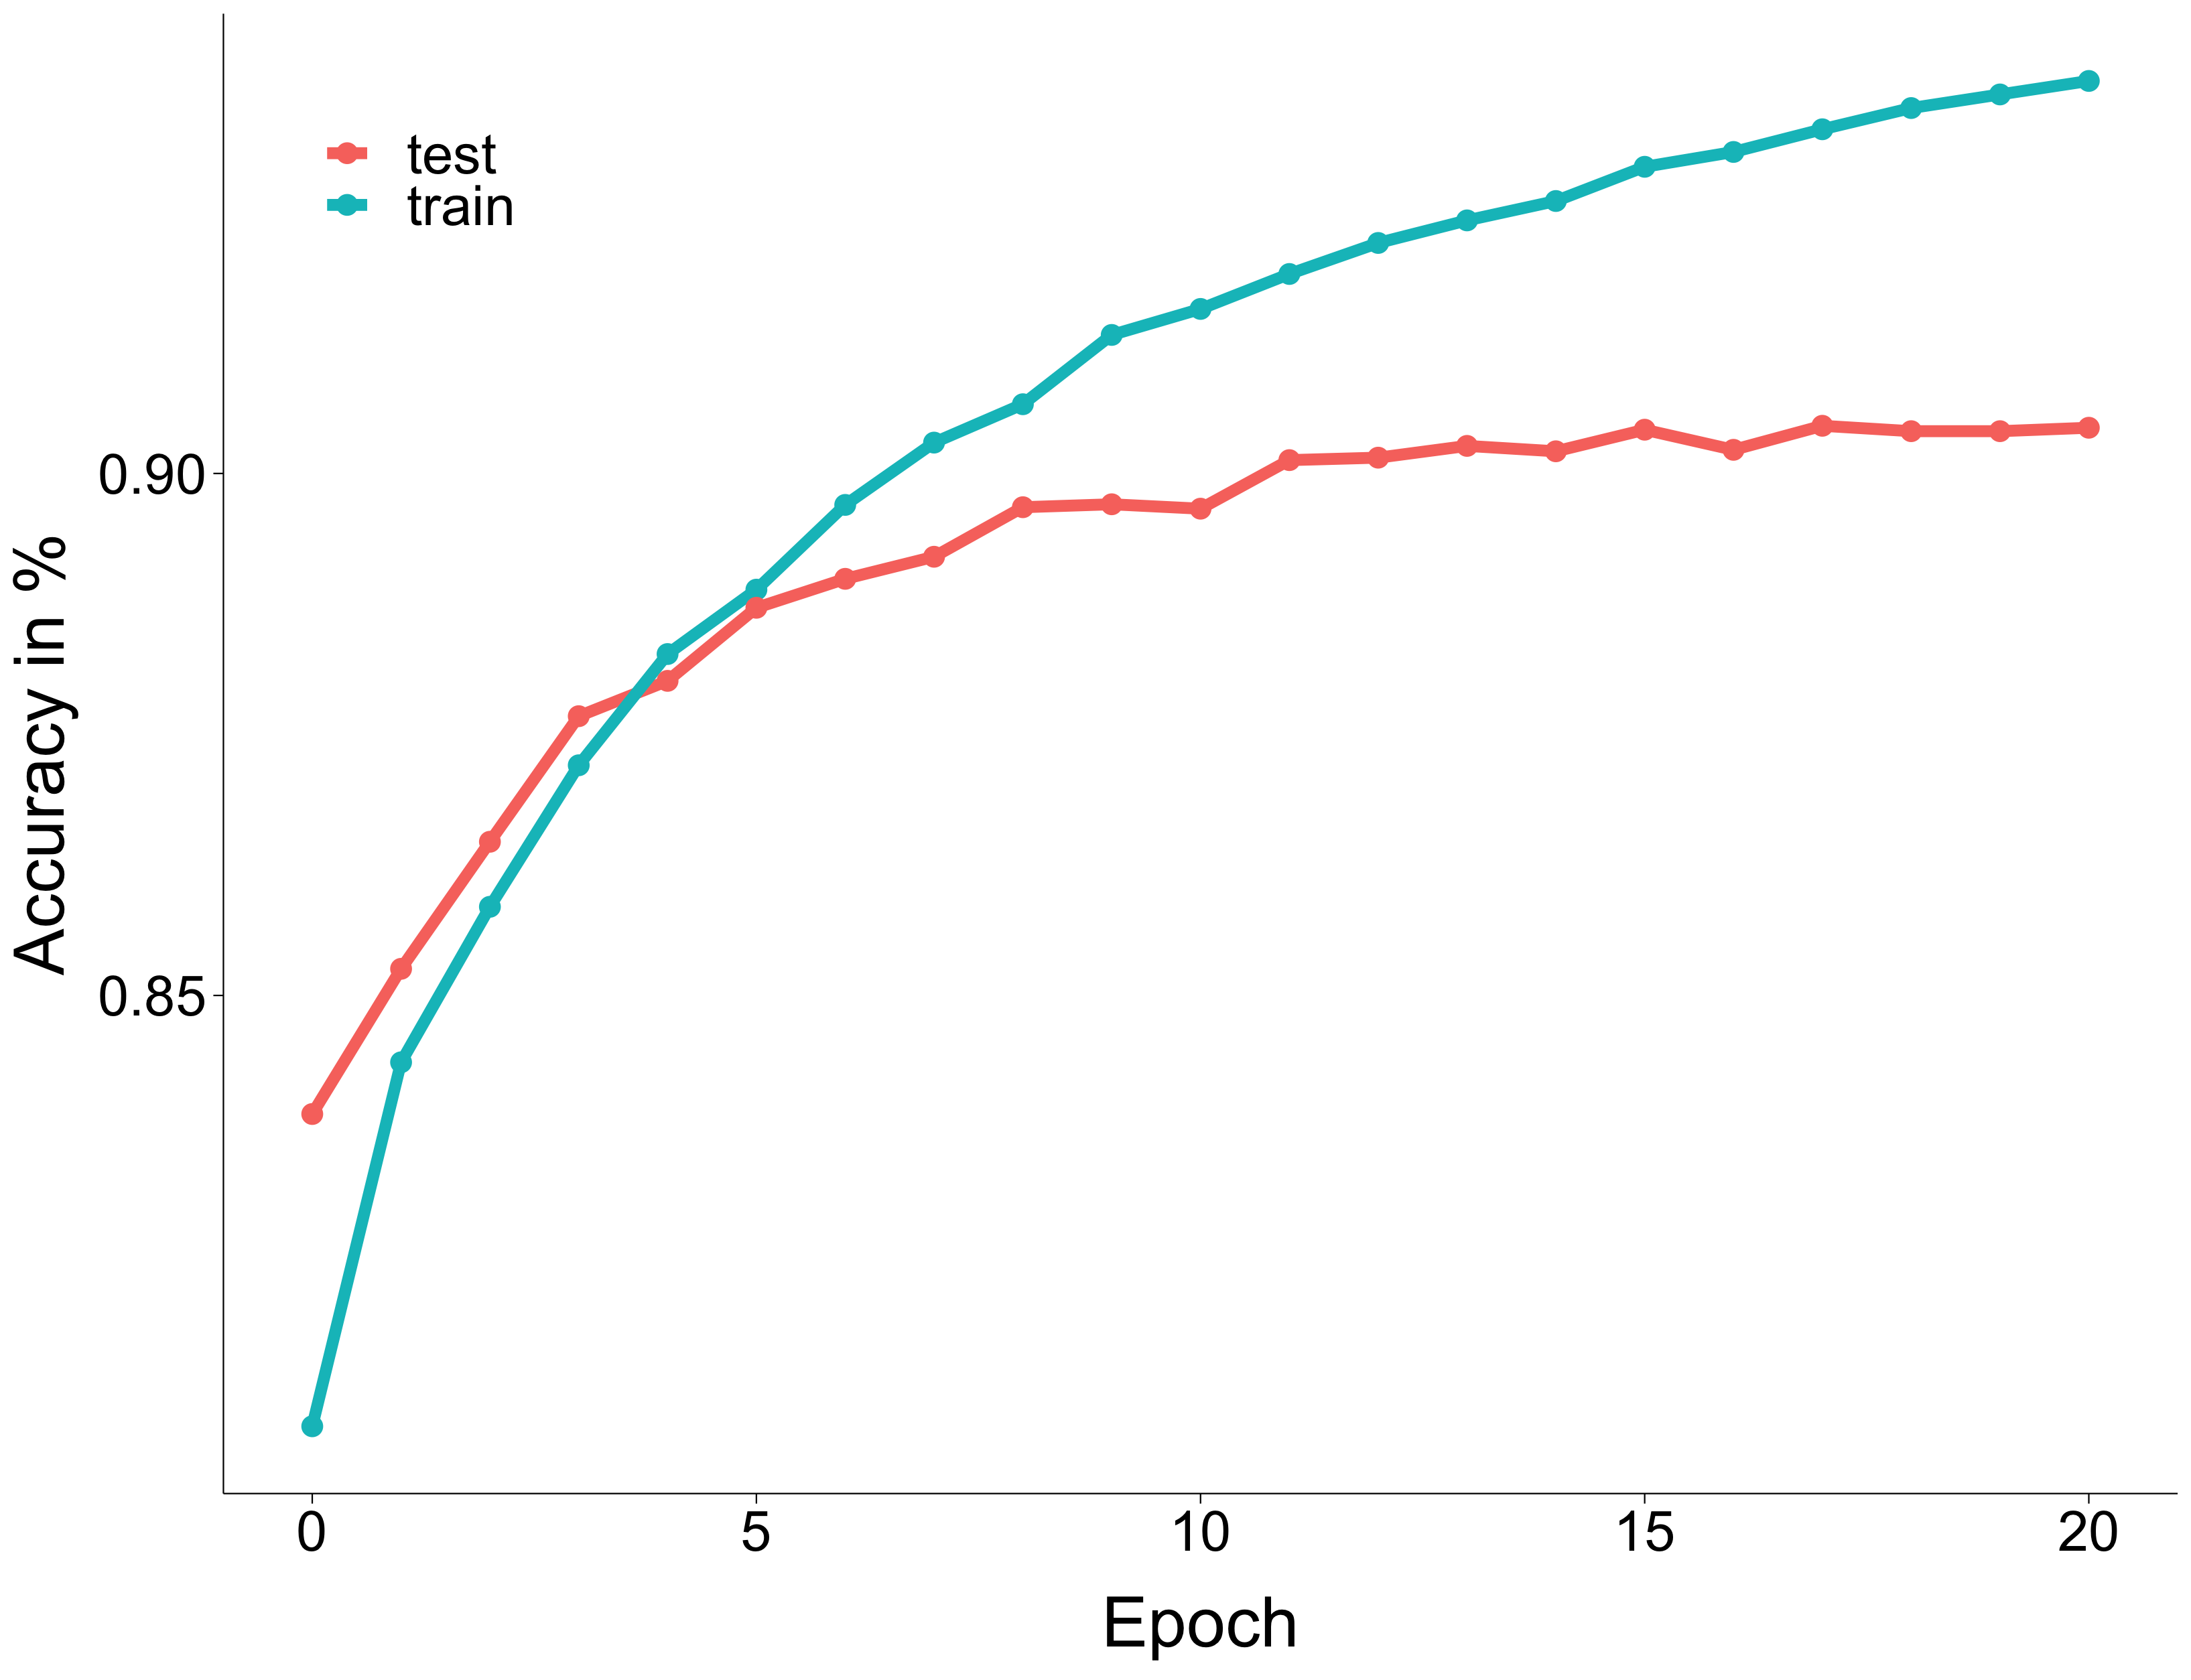
\includegraphics[width=\textwidth]{figures/plot_model_accuracies}
        \caption[Model accuracies on train and validation datasets.]{Model accuracies on train and validation datasets.}
        \label{fig:plot-model-accuracies}
    \end{minipage}
    \hfill
    \begin{minipage}[c]{.49\textwidth}
        \centering
        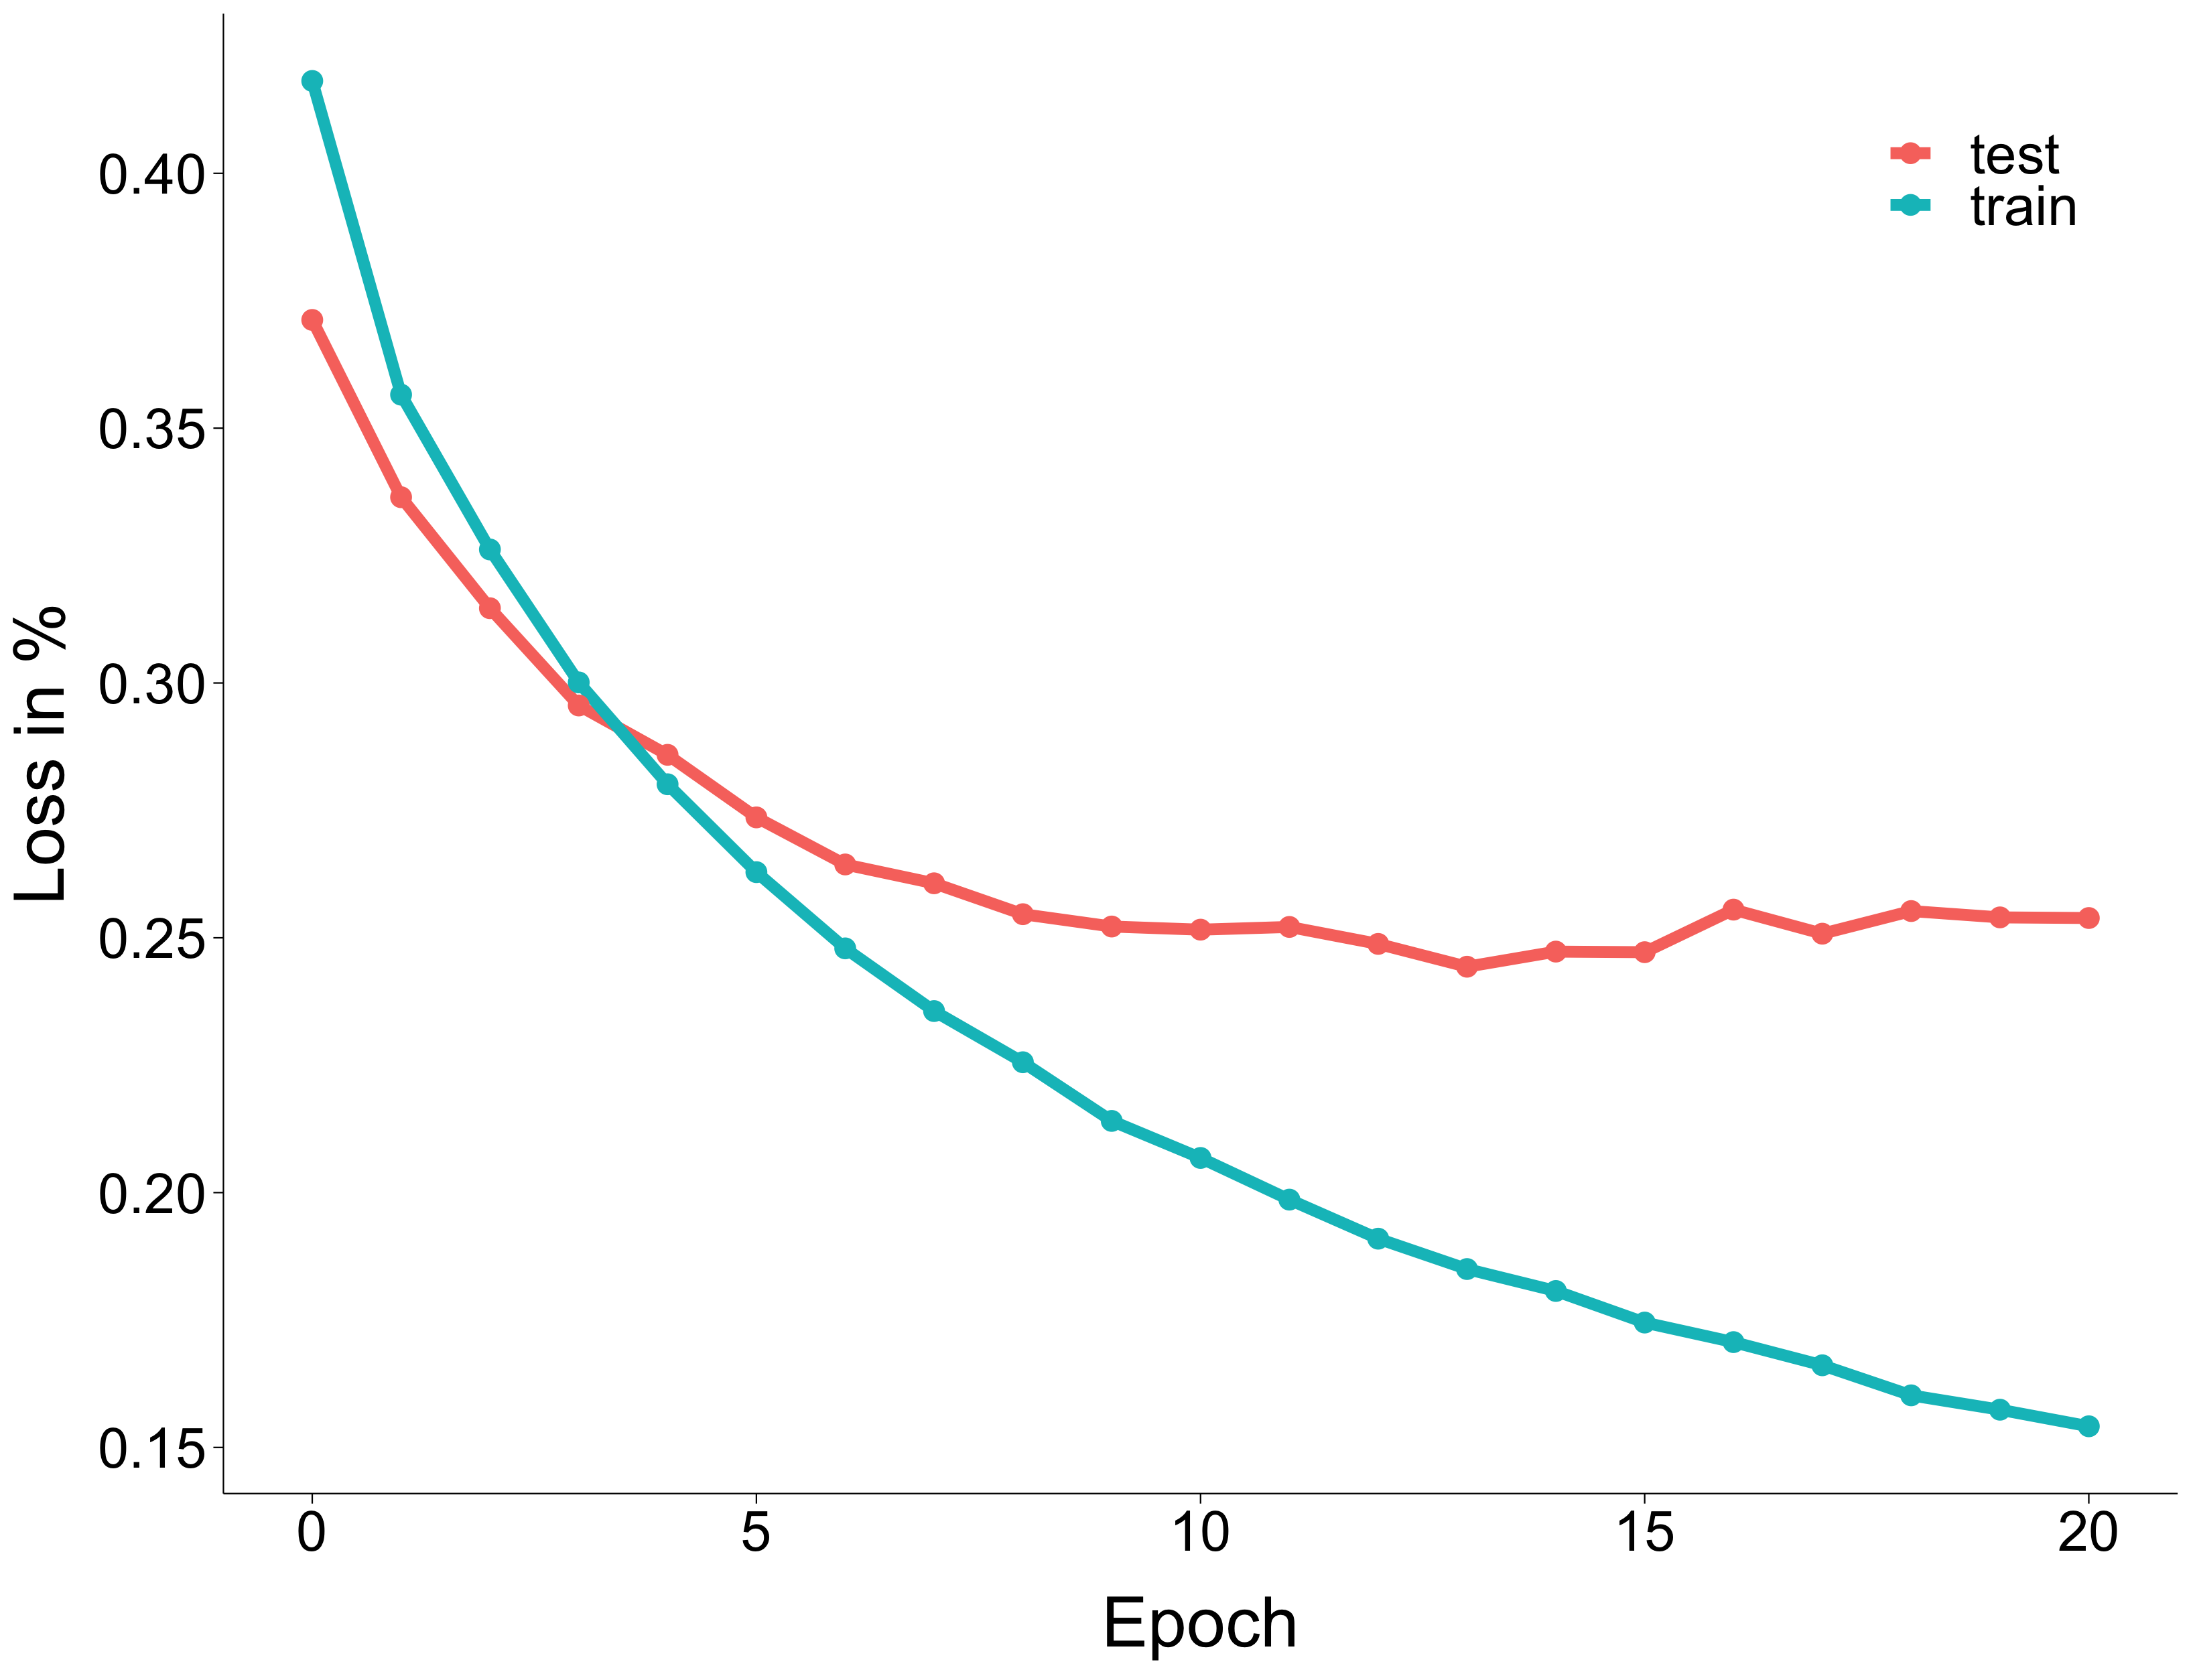
\includegraphics[width=\textwidth]{figures/plot_model_losses}
        \caption[Model losses on train and validation datasets.]{Model losses on train and validation datasets.}
        \label{fig:plot-model-losses}
    \end{minipage}
\end{figure}
%\begin{wrapfigure}{R}{0.65\textwidth}
%    \centering
%    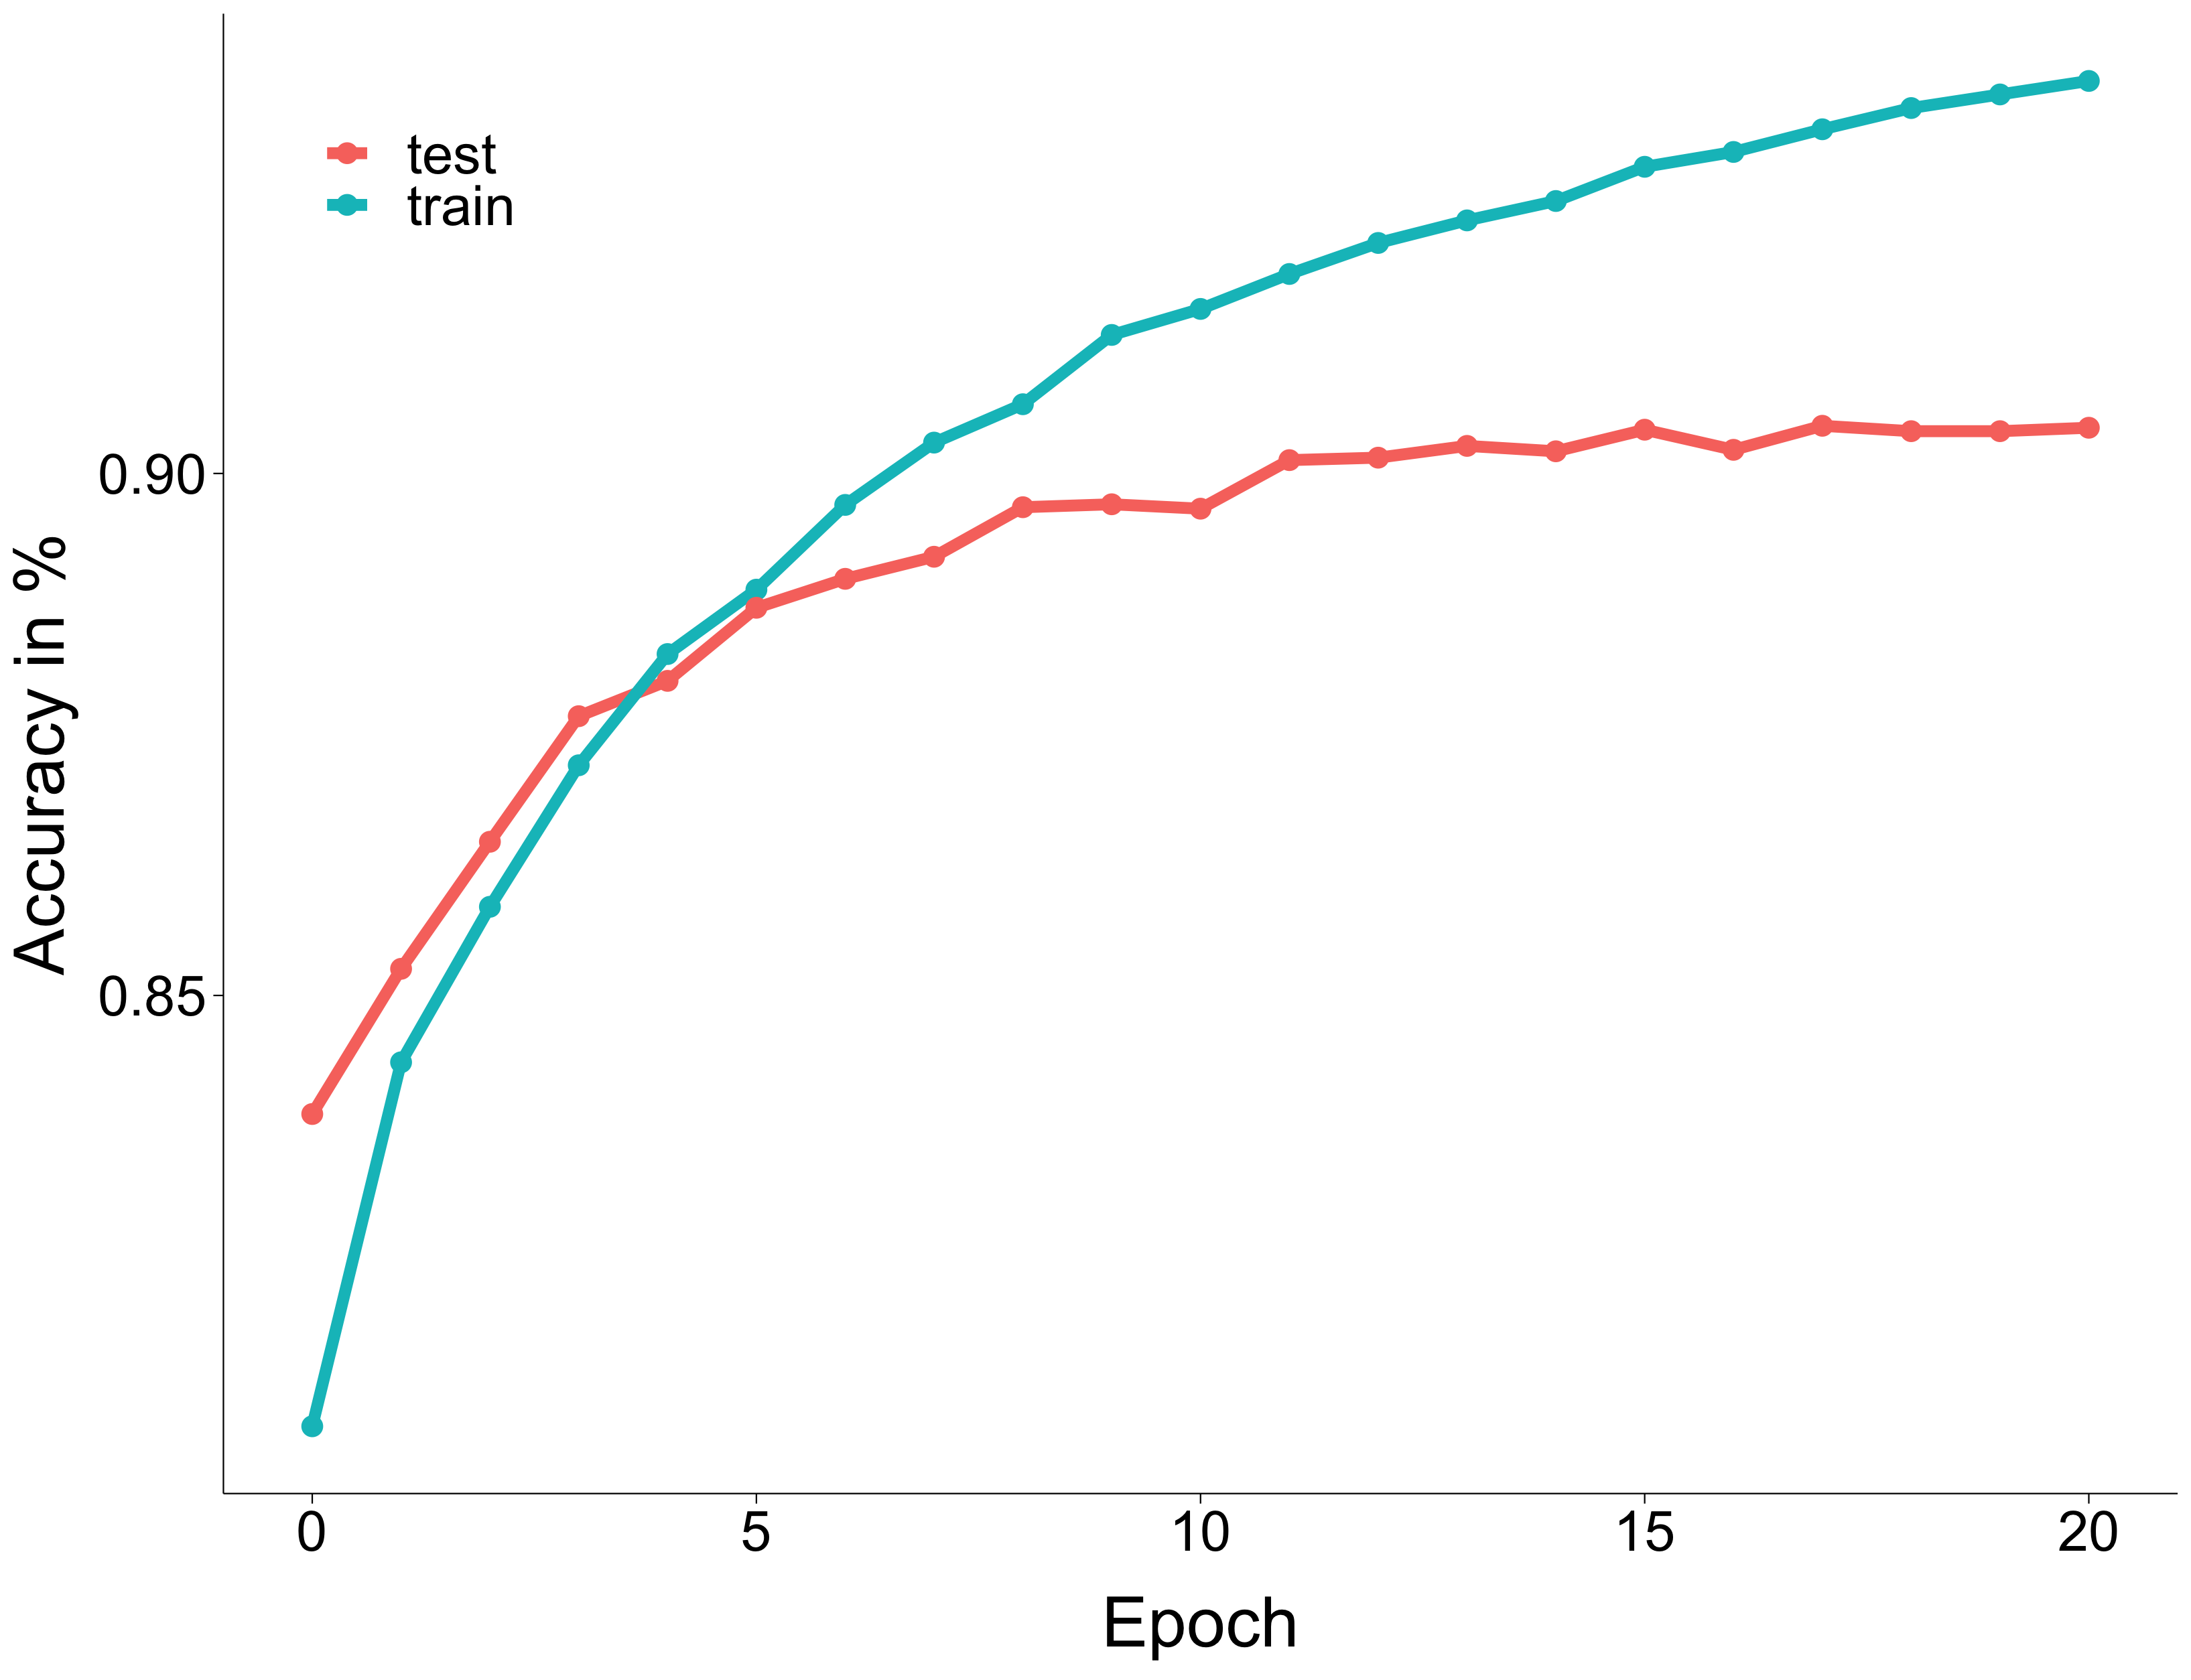
\includegraphics[width=0.6\textwidth]{figures/plot_model_accuracies}
%    \caption[Model accuracies on train and validation datasets.]{Model accuracies on train and validation datasets.}
%    \label{fig:plot-model-accuracies}
%\end{wrapfigure}
%\begin{wrapfigure}{R}{0.65\textwidth}
%    \centering
%    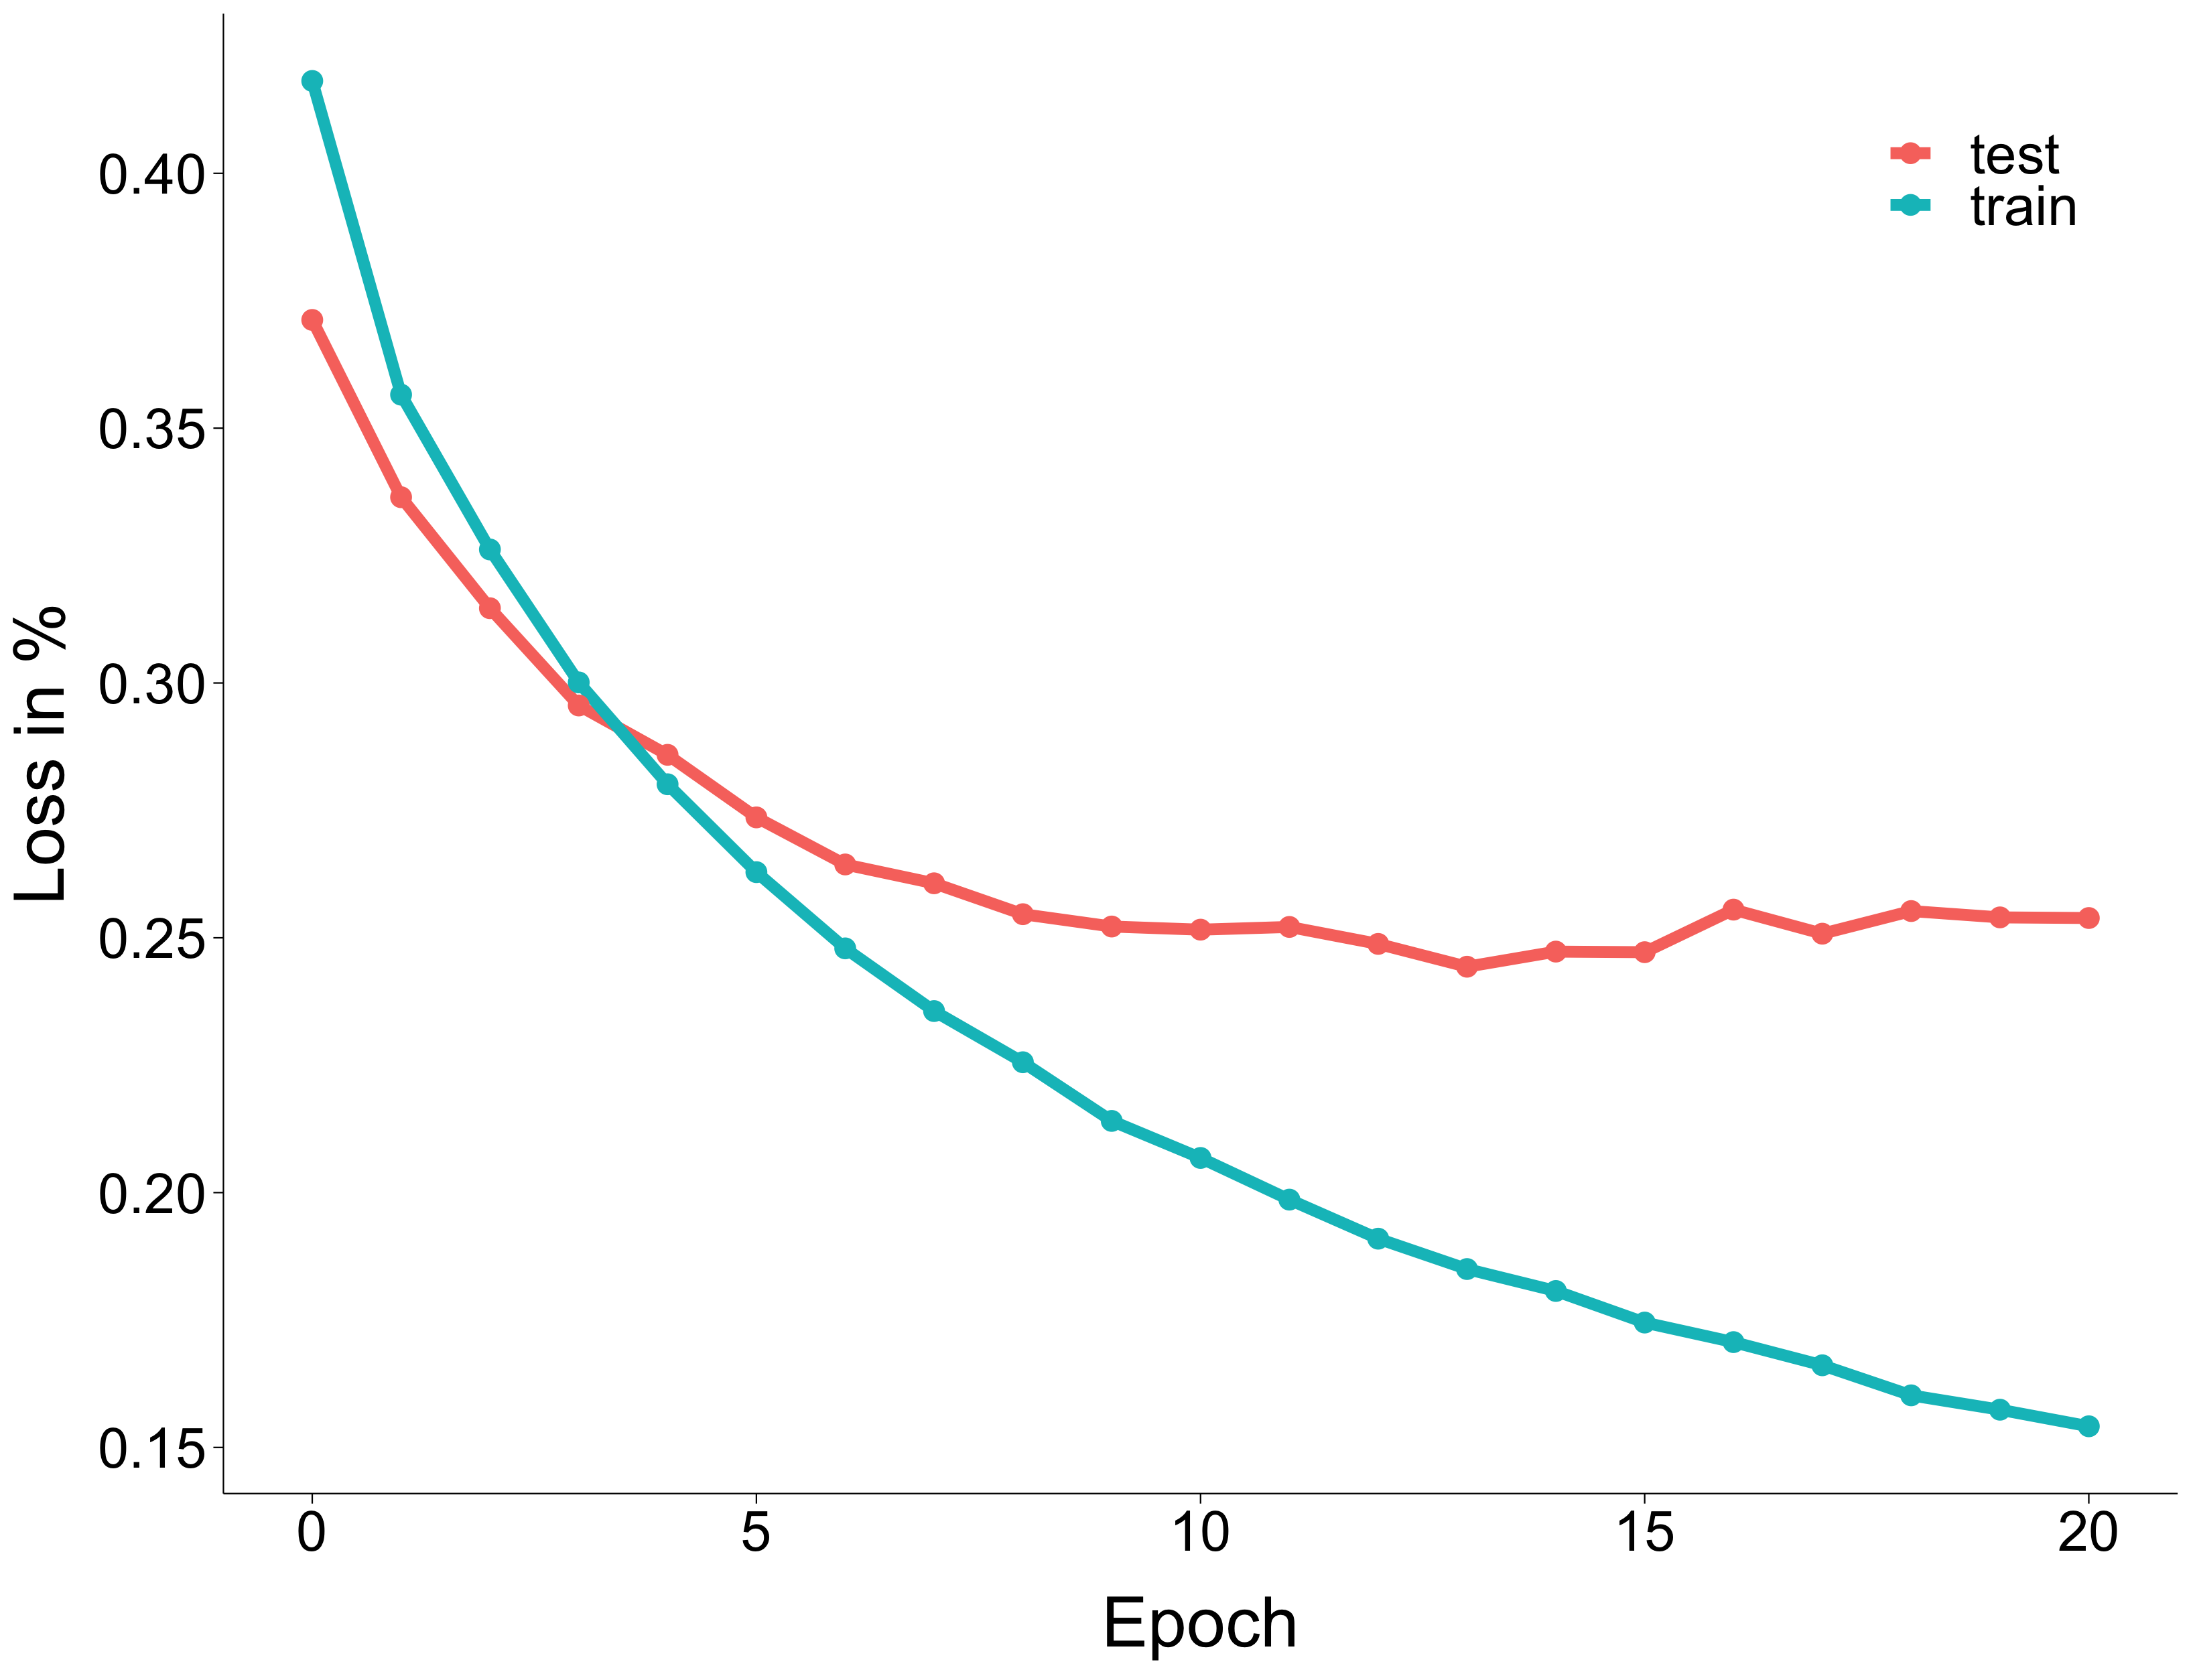
\includegraphics[width=0.6\textwidth]{figures/plot_model_losses}
%    \caption[Model losses on train and validation datasets.]{Model losses on train and validation datasets.}
%    \label{fig:plot-model-losses}
%\end{wrapfigure}

Accuracies (see Figure~\ref{fig:plot-model-accuracies}) were not rising significantly and losses (see Figure~\ref{fig:plot-model-losses}) for train and validation dataset departed after 21 epochs, so we stopped the training at this point.
We restored the weights from the best epoch (16) with an accuracy of 0.93 on the train and 0.90 on the test dataset.

\minisec{Predicting Story Character Genders}
The trained model was then used to predict the gender of each fictional character, their occurrences in the story and chapter were counted, and this information was then attached to the respective document.
In Section~\ref{sec:ner-token-classification}, we have already described how the story character names were extracted from the story texts.

To begin, we had to cleanse all the previously extracted story character names.
After some general clean-up operations, like removing special characters, numbers and whitespaces, we compared the names with the names from the training dataset.
If a match was found, the process was stopped immediately for that name, if not, we filtered words from the German \emph{DE-LIWC} dictionary~\citep{Meier2019LIWCDE-LIWC2015}.
For example, the name ``Glinda die Gute'' would become ``Glinda''.
Words were extracted from the \emph{LIWC 2015} poster in \emph{PDF} format using \emph{PyPDF2}\footnote{https://github.com/py-pdf/PyPDF2} and \emph{PDFMiner}\footnote{https://github.com/euske/pdfminer}.
Cleansed names with their cumulative occurrences were stored in the respective story document.

Given that iterating over each story in the corpus and predicting the genders of the story character names would have taken a significant amount of time, we split this process into several steps.

First, we extracted all story character names from the stories, removed any duplicates, and saved them to a separate \emph{CSV} file.
This newly created list was subsequently merged with the names from the training dataset and again duplicates were removed.
We then prepopulated additional information to the list, such as the gender and a probability value of 1.00 for all names from the training dataset.
This probability value was used to evaluate the confidence of the prediction, with 1.00 being the highest confidence and 0.00 being the lowest.

In the next step, this \emph{CSV} list was divided into 100 chunks with 2,800 stories each for the total 280,000 tagged stories.
Each chunk containing all the names from the 2,800 stories was then passed to the prediction model and the results with the predicted gender and probability were stored in a temporary data structure.
\begin{wrapfigure}{L}{0.65\textwidth}
    \centering
    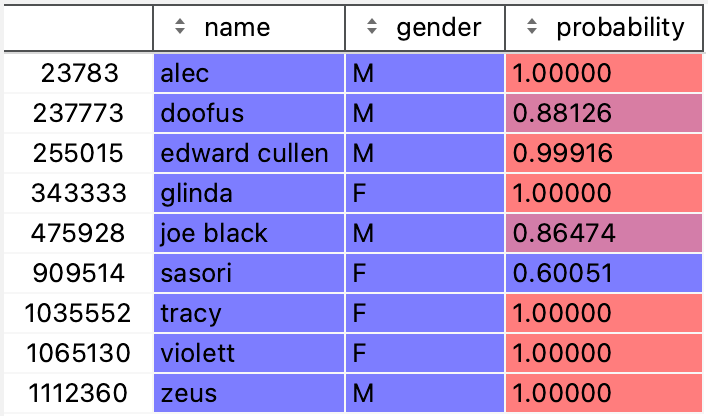
\includegraphics[width=0.55\textwidth]{figures/predicted_names_excerpt}
    \caption[Fragment of the \emph{CSV} list with the calculated gender of the names.]{Fragment of the \emph{CSV} list with the calculated gender of the names.}
    \label{fig:predicted-names-excerpt}
\end{wrapfigure}
After all chunks were processed, names with a low confidence of less than 0.80 and having at least one whitespace in the name were reprocessed.
The whitespaces were used to split the name into two parts, and the first part, a potential first name, was resent to the prediction model.
Finally, all prediction results were merged with the original list and saved in another \emph{CSV} file.
Figure~\ref{fig:predicted-names-excerpt} shows a fragment of this list to give an impression of what this looks like.

Utilizing this list, we iterated over all stories, comparing the names with the names from the prediction list.
Statistics showing the sum of all female, male, and indecisive names, along with their percentages and a female-to-male ratio, were then appended to the story document.
Whereas a ratio of 0.0 means that all decisive persons are female and 1.0 means that all are male, adapted from our one-hot coding for gender that we performed earlier for model training.
For example, a ratio of 0.7 means that the gender representation is rather male-dominated.

\chapter{Results and Discussion}\label{ch:results}

Utilizing all previously described and implemented methods, we analyzed the data and present the results in this chapter.
The results are divided into two sections: the first part is about general statistical analysis of the corpus, the second part is about the analysis of the gender representation.


\section{Corpus Analysis}\label{sec:corpus-analysis}

Fan Fiction archives were scraped over a time period of 7 months, from January 28 to August 23, 2022.
Updates for \emph{FF.de} database documents range over the full duration, while \emph{AO3} was processed over a period of 2 weeks, from July 25 to August 8, 2022.
This was due to the fact that German-language fan fiction is less common on \emph{AO3} in comparison and took therefore less time to scrape.
The corpus acquired consists of 412,923 stories, their chapters (1,955,923) and reviews (4,887,367), as well their respective authors (149,975) as depicted in Table~\ref{tab:corpus-overview}.

\begin{table}[htb]
    \renewcommand{\arraystretch}{1.5}
    \centering
    \begin{tabular}{lrrrr}
        \toprule
        \textbf{Archive} &
        \multicolumn{1}{c}{\textbf{Stories}} &
        \multicolumn{1}{c}{\textbf{Chapters}} &
        \multicolumn{1}{c}{\textbf{Users}} &
        \multicolumn{1}{c}{\textbf{Reviews}} \\
        \midrule
        \textbf{FF.de} & 394,848 & 1,885,066 & 135,726 & 4,849,646 \\
        \textbf{AO3}   & 18,075  & 70,857    & 14,249  & 37,721    \\
        \midrule
        \textbf{Total} & 412,923 & 1,955,923 & 149,975 & 4,887,367 \\
        \bottomrule
    \end{tabular}
    \caption[Corpus overview.]{Corpus overview.}
    \label{tab:corpus-overview}
\end{table}

\begin{table}[htb]
    \renewcommand{\arraystretch}{1.5}
    \centering
    \begin{tabular}{lrr}
        \toprule
        \multicolumn{1}{c}{\textbf{Fandom}} &
        \multicolumn{1}{c}{\cellcolor[HTML]{00576E}{\color[HTML]{FCFCF6} \textbf{FF.de}}} &
        \multicolumn{1}{c}{\cellcolor[HTML]{990000}{\color[HTML]{FFFFFF} \textbf{AO3}}} \\
        \midrule
        \addlinespace[.2em]\cellcolor[HTML]{990000}{\color[HTML]{FFFFFF} \textbf{Tatort}}                  & 644 (0.16\%)     & 2,978 (16.48\%) \\
        \addlinespace[.2em]\textbf{Harry Potter}                                                           & 54,405 (13.78\%) & 1,793 (9.92\%)  \\
        \addlinespace[.2em]\textbf{Music}                                                                  & 38,568 (9.77\%)  & 654 (3.62\%)    \\
        \addlinespace[.2em]\cellcolor[HTML]{00576E}{\color[HTML]{FCFCF6} \textbf{Naruto}}                  & 27,303 (6.91\%)  & 200 (1.11\%)    \\
        \addlinespace[.2em]\cellcolor[HTML]{990000}{\color[HTML]{FFFFFF} \textbf{Marvel}}                  & 5,311 (1.35\%)   & 1,234 (6.83\%)  \\
        \addlinespace[.2em]\cellcolor[HTML]{00576E}{\color[HTML]{FCFCF6} \textbf{Internet-Stars}}          & 17,830 (4.52\%)  & 50 (0.28\%)     \\
        \addlinespace[.2em]\cellcolor[HTML]{990000}{\color[HTML]{FFFFFF} \textbf{Canon}}                   & N/A              & 671 (3.71\%)    \\
        \addlinespace[.2em]\cellcolor[HTML]{00576E}{\color[HTML]{FCFCF6} \textbf{Twilight}}                & 13,734 (3.48\%)  & 45 (0.25\%)     \\
        \addlinespace[.2em]\cellcolor[HTML]{00576E}{\color[HTML]{FCFCF6} \textbf{One Piece}}               & 11,443 (2.90\%)  & 89 (0.49\%)     \\
        \addlinespace[.2em]\textbf{Sports}                                                                 & 11,440 (2.90\%)  & 663 (3.67\%)    \\
        \addlinespace[.2em]\cellcolor[HTML]{990000}{\color[HTML]{FFFFFF} \textbf{The Three Investigators}} & 1,251 (0.32\%)   & 509 (2.82\%)    \\
        \bottomrule
    \end{tabular}
    \caption[The top 7 fandoms on FF.de and AO3 respectively.]{The top 7 fandoms on FF.de and AO3 respectively. Individual appearances in the top fandoms are color-coded, while mutual appearances are not.}
    \label{tab:top-7-fandoms}
\end{table}

The lack of diversity in german fan fiction mentioned by \citet{Cuntz-Leng2015AGermany} in Section~\ref{sec:history-of-german-fan-fiction} can be confirmed.
Table~\ref{tab:top-7-fandoms} demonstrates that after 7 years, Harry Potter is still by a large margin the most popular fandom on \emph{FF.de}.
While in 2015 the top 7 fandom distributions have shifted only slightly, stories about musicians as \emph{One Piece}, \emph{One Direction} and \emph{Tokio Hotel} lost some popularity, likely due to the high fluctuation of overall approval ratings in the music industry.
With an increasing number of publications about celebrities from the Internet (YouTuber~\footnote{https://www.youtube.com}) and sports (mainly soccer), these fandoms have been overtaken.

An interesting observation is the very high number and overall share of stories about \emph{Tatort}, a German crime series, on \emph{AO3} compared to this fandom on \emph{FF.de}.
This is likely due to the fact that the fandom community for \emph{Tatort} established itself on \emph{AO3} and authors active in this rather publish their stories there.

The same assumption can safely be applied to fan fiction distribution as a whole as depicted in Table~\ref{tab:corpus-overview}.
Users publish their stories where their language specific fan base and community is located.
For German fanfiction, this is generally the \emph{FF.de} archive, but in rare cases on other platforms, such as in the instance of \emph{Tatort}.
This can explain the scarcity of German-language fan fiction on \emph{AO3}.
Another attempted explanation is the tendency, mentioned in Section~\ref{sec:history-of-german-fan-fiction}~\citep{Cuntz-Leng2015AGermany}, to migrate to fan fiction written in English, even as a non-native speaker.

Like \citet{Schmidt2021TowardsOwn} for AO3, we also observe regarding the supposedly strongly intertwined anime fan fiction in Germany that the most popular anime fandom in our corpus is \emph{Naruto} with only 27,503 stories and a share of 6.66\%.
Even in commonly male-dominated genres, there is a preponderance of female writers.

Also worth mentioning in this context are the works about stories by Karl May, who, according to \citet{Cuntz-Leng2015AGermany}, is said to have been directly responsible for the emergence and development of the German fan fiction scene in the 19th century.
This so-called phenomenon seems to have died before the establishment of online archives, because the number of publications about Karl May stories on \emph{FF.de} is only 204 (0.05\%) and on \emph{AO3} 46 (0.25\%).

\begin{table}[htb]
    \renewcommand{\arraystretch}{1.25}
    \centering
    \begin{tabular}{lrrrr}
        \toprule
        \multicolumn{1}{c}{\textbf{Genre}} &
        \multicolumn{1}{c}{\textbf{Sentences}} &
        \multicolumn{1}{c}{\textbf{Words}} &
        \multicolumn{1}{c}{\textbf{Letters}} &
        \multicolumn{1}{c}{\textbf{Characters}} \\
        \midrule
        \textbf{Musicals}             & 19,911 & 243,903 & 1,221,731 & 1,523,534 \\
        \textbf{Books \& Literature}  & 1,777  & 21,389  & 107,618   & 133,041   \\
        \textbf{Crossover}            & 1,037  & 9,897   & 46,485    & 58,682    \\
        \textbf{Other Media}          & 334    & 3,263   & 16,298    & 20,096    \\
        \textbf{Cartoons \& Comics}   & 318    & 3,230   & 16,111    & 20,588    \\
        \textbf{Movies}               & 197    & 3,155   & 15,256    & 19,193    \\
        \textbf{Celebrities}          & 110    & 1,351   & 6,510     & 8,210     \\
        \textbf{Anime \& Manga}       & 101    & 812     & 4,248     & 5,460     \\
        \textbf{Video Games}          & 98     & 1,423   & 7,672     & 9,363     \\
        \textbf{Tabletop \& RPGs}     & 70     & 788     & 3,746     & 4,719     \\
        \textbf{TV-Shows \& Podcasts} & 33     & 224     & 1,016     & 1,440     \\
        \midrule
        \textbf{Total}                & 157    & 1,763   & 8,685     & 10,881    \\
        \bottomrule
    \end{tabular}
    \caption[Medians for sentences, words, letters and characters for each genre.]{Medians for sentences, words, letters and characters for each genre.}
    \label{tab:median-counts}
\end{table}

Table~\ref{tab:median-counts} shows the median values for the number of sentences, words, letters and characters for each genre.
While publications about musicals are rather unpopular, with a share of only 0.68\% (2,795 stories), they are the longest, with the highest number of sentences, words, letters and characters.
In this regard, the statistics about \emph{Books \& Literature} and crossovers can be considered more significant, which in the case of the latter often includes works about written texts as well, with a total share of 28.21\% (116,481) and the second longest with a median of 31,286 words.
The original works on which these stories are based are also typically written in a fairly lengthy and detailed manner.
Consequently, the fan fictions that refer to them are often written in the same style and reflect this in their length as well.
Works about games and \emph{TV-Shows \& Podcasts} are the shortest published stories on average.

% TODO: tab:story-pairings
% explain pairing types
% ``characters and observed an overwhelming amount of male-male relationships in fan fiction (91.99%; Tosenberger (2008); Hellekson & Busse (2006); Duggan (2017), Kleindienst & Schmidt (2020) ) compared to the source material.''

\begin{table}[htb]
    \renewcommand{\arraystretch}{1.5}
    \centering
    \begin{tabular}{lrr}
        \toprule
        \textbf{Pairing} &
        \multicolumn{1}{c}{\textbf{Frequency}} &
        \multicolumn{1}{c}{\textbf{Mean}} \\
        \midrule
        \textbf{Generic} & 276,188 & 66.50\% \\
        \textbf{M/M}     & 117,051 & 28.18\% \\
        \textbf{F/M}     & 14,784  & 3.56\%  \\
        \textbf{F/F}     & 2,826   & 0.68\%  \\
        \textbf{Multi}   & 2,702   & 0.65\%  \\
        \textbf{N/A}     & 1,059   & 0.25\%  \\
        \textbf{Diverse}   & 693     & 0.17\%  \\
        \bottomrule
    \end{tabular}
    \caption{Comparison of story pairings sorted by frequency.}
    \label{tab:story-pairings}
\end{table}

Pairings in fan fiction are classifications of stories referring to the romantic relationship between characters.
According to Table~\ref{tab:story-pairings} the most common pairing is the generic one, which is used for stories where relationships do not exist at all or are not addressed.
The second most common pairing is \emph{M/M} or \emph{MaleSlash}.
It implies that romantic relationships are present in the story and are also thematized.
Primarily, it is about romantic relationships between men.
The opposing classification of this is \emph{F/F} or \emph{FemSlash}, which is used for stories about romantic relationships between women.
While \emph{F/M} describes heterosexual relationships, \emph{Diverse} relationships that can not be classified and \emph{Multi} relationships that do involve multiple previously defined pairings without a predominant one.

Potential reasons for the share of \emph{MaleSlash} stories being so high are discussed later in this chapter.

After this general statistical analysis of the corpus, the focus in the following section shifts towards the representation of gender in fan fiction.


\section{Gender Representation in Fan Fiction}\label{sec:gender-representation-in-fan-fiction}

Previous research has shown that women are underrepresented in a variety of media forms~\citep{Collins2011ContentGo}.
In popular films, for example, men provide more than two-thirds of the speaking roles~\citep{Neville2019FewerFilms}.
This section examines whether this can also be observed in the media form of fan fiction.
The subject of the investigation is the previously acquired corpus on German fan fiction.

\subsection{Analyzing Character Genders}\label{subsec:analyzing-character-genders}

To analyze gender representation in German fan fiction, we used with \emph{Flair}\citep{Akbik2019FLAIR:NLP} a named entity recognition model to extract the story characters' names from the stories and trained an LSTM model to predict their respective gender, as outlined in Section~\ref{sec:determine-character-name-genders}.
The general results of this approach are presented in Table~\ref{tab:gender-representation}, which compares the number of male, female, and indecisive story characters, that is, story characters whose prediction did not reach a confidence of 0.80\% or higher.

\begin{table}[htb]
    \renewcommand{\arraystretch}{1.5}
    \centering
    \begin{tabular}{lrrrr}
        \toprule
        \textbf{Archive} &
        \multicolumn{1}{c}{\textbf{Ratio}} &
        \multicolumn{1}{c}{\textbf{Males}} &
        \multicolumn{1}{c}{\textbf{Females}} &
        \multicolumn{1}{c}{\textbf{Indecisives}} \\
        \midrule
        \textbf{FF.de} & 0.63 & 36,000,856 (60.85\%) & 19,471,225 (32.91\%) & 3,695,846 (6.25\%) \\
        \textbf{AO3}   & 0.74 & 579,925 (71.63\%)    & 189,421 (23.40\%)    & 40,212 (4.97\%)    \\
        \midrule
        \textbf{Total} & 0.63 & 36,580,781           & 19,660,646           & 3,736,058          \\
        \bottomrule
    \end{tabular}
    \caption[Gender representation of \emph{FF.de} and \emph{AO3}.]{Gender representation of \emph{FF.de} and \emph{AO3}.
    Ratio is using the arithmetic mean and depicts only Male and Female proportions with 1 = all male and 0 = all female.
    Shown percentages are on a per-archive basis.}
    \label{tab:gender-representation}
\end{table}

It can be observed that most characters could be predicted sufficiently with only about 5\% of all characters being indecisive.
The majority of characters appearing in fictional stories are male at 60.85\% on \emph{FF.de} and even more so on \emph{AO3} at 71.63\%.
Since the number of stories on \emph{AO3} is significantly lower and tends to be less diverse with fandoms such as \emph{Tatort} accounting for a large proportion of published texts, the percentage shown for \emph{FF.de} is likely to be the relevant one, as the unchanged overall ratio suggests.

Consequently, a distinction between the two archives in this context is rather unnecessary and both archives can be considered as a whole.
Statistics on characteristics that do not achieve a confidence of at least 0.80\% (indecisives) are omitted in the following analysis.
Furthermore, the ratio will always represent the distribution of male and female units with 1 = all male and 0 = all female.

\begin{table}[htb]
    \centering
    \begin{tabular}{lcrrr}
        \toprule
        \textbf{Fandom w/ Genre} &
        \multicolumn{1}{c}{\textbf{Ratio}} &
        \multicolumn{1}{c}{\textbf{Males}} &
        \multicolumn{1}{c}{\textbf{Females}} \\
        \midrule
        \textbf{Harry Potter}       & \cellcolor[HTML]{96b7ed}                       &                              &                           \\
        \emph{Books \& Literature}  & \multirow{-2}{*}{\cellcolor[HTML]{96b7ed}0.69} & \multirow{-2}{*}{13,296,037} & \multirow{-2}{*}{720,302} \\
        \addlinespace[.2em]
        \textbf{Musik}              & \cellcolor[HTML]{a3c0f0}                       &                              &                           \\
        \emph{Celebrities}          & \multirow{-2}{*}{\cellcolor[HTML]{a3c0f0}0.66} & \multirow{-2}{*}{978,215}    & \multirow{-2}{*}{379,515} \\
        \addlinespace[.2em]
        \textbf{Naruto}             & \cellcolor[HTML]{c9daf8}                       &                              &                           \\
        \emph{Anime \& Manga}       & \multirow{-2}{*}{\cellcolor[HTML]{c9daf8}0.57} & \multirow{-2}{*}{571,593}    & \multirow{-2}{*}{393,172} \\
        \addlinespace[.2em]
        \textbf{Supernatural}       & \cellcolor[HTML]{3c78d8}                       &                              &                           \\
        \emph{TV-Shows \& Podcasts} & \multirow{-2}{*}{\cellcolor[HTML]{3c78d8}0.90} & \multirow{-2}{*}{294,194}    & \multirow{-2}{*}{52,332}  \\
        \addlinespace[.2em]
        \textbf{Marvel}             & \cellcolor[HTML]{749fe5}                       &                              &                           \\
        \emph{Movies}               & \multirow{-2}{*}{\cellcolor[HTML]{749fe5}0.77} & \multirow{-2}{*}{318,954}    & \multirow{-2}{*}{107,142} \\
        \addlinespace[.2em]
        \textbf{Crossover}          & \cellcolor[HTML]{acc6f2}                       &                              &                           \\
        \emph{Crossover}            & \multirow{-2}{*}{\cellcolor[HTML]{acc6f2}0.64} & \multirow{-2}{*}{1,068,512}  & \multirow{-2}{*}{506,279} \\
        \addlinespace[.2em]
        \textbf{Online Games}       & \cellcolor[HTML]{c5d8f8}                       &                              &                           \\
        \emph{Video Games}          & \multirow{-2}{*}{\cellcolor[HTML]{c5d8f8}0.58} & \multirow{-2}{*}{365,981}    & \multirow{-2}{*}{266,543} \\
        \addlinespace[.2em]
        \textbf{Marvel}             & \cellcolor[HTML]{4e84dc}                       &                              &                           \\
        \emph{Cartoons \& Comics}   & \multirow{-2}{*}{\cellcolor[HTML]{4e84dc}0.86} & \multirow{-2}{*}{45,670}     & \multirow{-2}{*}{5,157}   \\
        \addlinespace[.2em]
        \textbf{Tanz der Vampire}   & \cellcolor[HTML]{a7c3f1}                       &                              &                           \\
        \emph{Musicals}             & \multirow{-2}{*}{\cellcolor[HTML]{a7c3f1}0.65} & \multirow{-2}{*}{207,777}    & \multirow{-2}{*}{94,481}  \\
        \addlinespace[.2em]
        \textbf{Canon}              & \cellcolor[HTML]{c5d8f8}                       &                              &                           \\
        \emph{Other Media}          & \multirow{-2}{*}{\cellcolor[HTML]{c5d8f8}0.58} & \multirow{-2}{*}{12,146}     & \multirow{-2}{*}{3,308}   \\
        \addlinespace[.2em]
        \textbf{Das Schwarze Auge}  & \cellcolor[HTML]{b0c9f3}                       &                              &                           \\
        \emph{Tabletop \& RPGs}     & \multirow{-2}{*}{\cellcolor[HTML]{b0c9f3}0.63} & \multirow{-2}{*}{19,672}     & \multirow{-2}{*}{16,806}  \\
        \bottomrule
    \end{tabular}
    \caption[Gender representation of characters in top fandoms per genre.]{Gender representation of characters in each top fandom per genre. Sorted by their amount of stories in descending order. Ratio depicts only Male and Female proportions with 1 = all male and 0 = all female.}
    \label{tab:gender-representation-fandoms}
\end{table}
Table~\ref{tab:gender-representation-fandoms} illustrates this by listing the top fandoms for each genre, sorted by the popularity of the genre.

Three fandoms stand out among these: Supernatural, the Marvel cinematic universe, as well as their carton and comic counterpart.
They all have an even larger amount of male story characters compared to the rest.

In the case of the television series Supernatural, this can be explained by the study conducted by \citet{Kleindienst2020InvestigatingSupernatural} on AO3.
They found that the texts in this fandom contained male-male relationships at an overwhelming rate of 91.99\%.
This trend also seems to be applicable to the \emph{FF.de} corpus, though most pairings for \emph{Supernatural} are declared as \emph{Generic} (58.79\%) rather than male-male (38.92\%).
This will be discussed in more detail later on.

Although there has been an increase in the number of female characters in the \emph{Marvel Universe}, the overall number is still quite low, with a total percentage of 19.88\%, according to \citet{Ray2020GenderViolence}$'$s research on the \emph{Marvel Cinematic Universe}.
This scarcity of female characters in the canon, as well as an already strong tendency towards male characters in fan fiction in general, has likely led to this heavily male biased ratio.

\subsection{Analyzing Gender-Specific Pronouns}\label{subsec:analyzing-gender-specific-pronouns}

Seen across all fan fiction genres, the distribution of used feminine and masculine personal pronouns is fairly even as shown in Table~\ref{tab:pronouns-distribution}.
This confirms the tendency that has already been identified with regard to the predominance of male characters in the stories of this community.
A correlation was to be expected, since the characters introduced in the story are addressed with personal pronouns to the same degree they are occurring.

\begin{table}[htb]
    \renewcommand{\arraystretch}{1.25}
    \centering
    \begin{tabular}{lrrr}
        \toprule
        \multicolumn{1}{c}{\textbf{Genre}} &
        \multicolumn{1}{c}{\textbf{Feminine}} &
        \multicolumn{1}{c}{\textbf{Masculine}} &
        \multicolumn{1}{c}{\textbf{Total}} \\
        \midrule
        \textbf{Books \& Literature}  & \cellcolor[HTML]{F980F6}38.05\% & \cellcolor[HTML]{8DB4F0}61.95\% & 64,144,827 \\
%        \addlinespace[.2em]
        \textbf{TV-Shows \& Podcasts} & \cellcolor[HTML]{FA8BF6}35.96\% & \cellcolor[HTML]{8AB1EF}64.04\% & 27,431,159 \\
%        \addlinespace[.2em]
        \textbf{Anime \& Manga}       & \cellcolor[HTML]{FB98F6}33.55\% & \cellcolor[HTML]{85AEEF}66.45\% & 18,979,393 \\
%        \addlinespace[.2em]
        \textbf{Movies}               & \cellcolor[HTML]{F982F6}37.65\% & \cellcolor[HTML]{8DB3F0}62.35\% & 8,948,841  \\
%        \addlinespace[.2em]
        \textbf{Video Games}          & \cellcolor[HTML]{F982F6}37.66\% & \cellcolor[HTML]{8DB3F0}62.34\% & 8,765,844  \\
%        \addlinespace[.2em]
        \textbf{Celebrities}          & \cellcolor[HTML]{FFDDF5}20.71\% & \cellcolor[HTML]{6D9EEB}79.29\% & 6,469,078  \\
%        \addlinespace[.2em]
        \textbf{Cartoons \& Comics}   & \cellcolor[HTML]{F87AF6}39.08\% & \cellcolor[HTML]{8FB5F0}60.92\% & 4,500,338  \\
%        \addlinespace[.2em]
        \textbf{Crossover}            & \cellcolor[HTML]{F986F6}36.86\% & \cellcolor[HTML]{8BB2F0}63.14\% & 2,640,782  \\
%        \addlinespace[.2em]
        \textbf{Musicals}             & \cellcolor[HTML]{F97FF6}38.20\% & \cellcolor[HTML]{8EB4F0}61.80\% & 1,564,273  \\
%        \addlinespace[.2em]
        \textbf{Tabletop \& RPGs}     & \cellcolor[HTML]{F76DF7}41.39\% & \cellcolor[HTML]{94B8F1}58.61\% & 347,633    \\
%        \addlinespace[.2em]
        \textbf{Other Media}          & \cellcolor[HTML]{FDC1F5}25.94\% & \cellcolor[HTML]{77A5ED}74.06\% & 282,224    \\
%        \addlinespace[.2em]
        \bottomrule
    \end{tabular}
    \caption[Distribution of feminine and masculine personal pronouns per genre.]{Distribution of feminine and masculine personal pronouns per genre.}
    \label{tab:pronouns-distribution}
    % TODO: add character gender ratios?
\end{table}

Moreover, it can be assumed that this ratio would presumably have to shift even further in the direction of the masculine pronouns.
This is due to the fact that we previously defined the German ``sie'' (she) as a feminine personal pronoun, although it can also refer to the third-person plural or ``you'' in the polite form.
However, this does not apply analogously to the German ``er'' (he), which is used exclusively for the masculine third-person singular.

The genres \emph{Celebrities} and \emph{Other Media} stand out in comparison with an even greater discrepancy between the use of feminine and masculine pronouns.
To this extent, this discrepancy could not be observed before when comparing the character genders (see Table~\ref{tab:gender-representation-fandoms}).
% TODO: explanation?
\emph{Other Media} is a genre exclusive to \emph{AO3}, much of which consists of canons or original works.
In this case, the discrepancy was previously seen in the gender ratio of the characters.
This gives the impression, and also confirms the thesis of \citet{Milli2016BeyondFanfiction}, that canonical works are leaning even more towards a male-dominated narrative, in spite of the fact that only a quite small sample can be referred to for comparison.

\subsection{Adding the User's Sex to the Ratio}\label{subsec:user-sex-comparisons}

\citet{Duggan2020WhoAO3} previously stated that the sex of authors was directly dependent on the portrayal of gender roles in their stories.
While they analyzed story paratexts and profile biographies on \emph{AO3} for the \emph{Harry Potter} fandom to extract their writer's sex, we were able to use the information provided by the users themselves, since users can submit it to their profiles.
Due to their approach Duggan had a very small sample size of 1,800 users of which only 265 provided extractable information regarding their gender.
As a consequence, we limit our analysis to the sex of \emph{FF.de} users, but this is negligible in respect to the rather small number of german stories on \emph{AO3} in any case.
Users have the option to specify in their profile whether they consider themselves ``weiblich'' (female), ``männlich'' (male) or ``divers'' (diverse).
While Duggan extracted this information, we had to trust the users to provide it correctly which could lead to deviations.

\begin{table}[htb]
    \renewcommand{\arraystretch}{1.5}
    \centering
    \begin{tabular}{lrrrr}
        \toprule
        \multicolumn{1}{c}{\textbf{User's Sex}} &
        \multicolumn{1}{c}{\textbf{Frequency}} &
        \multicolumn{1}{c}{\textbf{Authors}} &
        \multicolumn{1}{c}{\textbf{Reviewers}} &
        \multicolumn{1}{c}{\textbf{Age}} \\
        \midrule
        \textbf{Female}  & 87,784 (64.68\%) & 72,959 (68.04\%) & 51,084 (67.89\%) & 26.89 \\
        \textbf{Male}    & 7,834 (5.77\%)   & 6,291 (5.87\%)   & 4,521 (6.01\%)   & 27.98 \\
        \textbf{Diverse} & 671 (0.49\%)     & 511 (0.48\%)     & 450 (0.60\%)     & 23.12 \\
        \textbf{N/A}     & 39,437 (29.06\%) & 27,463 (25.61\%) & 19,185 (25.50\%) & 27.10 \\
        \midrule
        \textbf{Total}   & 135,726          & 107,224          & 75,240           & 26.97 \\
        \bottomrule
    \end{tabular}
    \caption[Frequencies of FF.de users regarding their sex.]{Frequencies of FF.de users regarding their sex. The distinction between Authors and Reviewers ist not mutual exclusive, but users are unique for each category. Age is the arithmetic mean of all users for the respective sex.}
    \label{tab:user-gender-frequencies}
\end{table}

In Table~\ref{tab:user-gender-frequencies}, we can observe that with about 70.94\% the majority of users state their sex.
For all sexes, users tend to author stories more likely than review any.
% Milli: ``Furthermore, they identified that more than half of the fan-authors (52\%) are in return reviewers of other works.''

We therefore cannot confirm Duggans assessment towards the diversity of users, with only 0.49\% stating ``diverse'', but the one towards an overwhelming majority of female writers and readers (about 50\%) and even surpass this with about 65\% female users.
This is contrary to \citet{Fast2016ShirtlessCommunity} findings on high-level gender statistics from \emph{Wattpad}\footnote{https://www.wattpad.com}, which state that the majority of fan fiction creators tend to be male, at around 54\%.

\begin{table}[htb]
    \renewcommand{\arraystretch}{1.5}
    \centering
    \begin{tabular}{lrrrrr}
        \toprule
        \multicolumn{1}{c}{\textbf{Genre}} &
        \multicolumn{1}{c}{\textbf{Frequency}} &
        \multicolumn{1}{c}{\textbf{Females}} &
        \multicolumn{1}{c}{\textbf{Males}} &
        \multicolumn{1}{c}{\textbf{Diverse}} &
        \multicolumn{1}{c}{\textbf{N/A}} \\
        \midrule
        \textbf{Anime \& Manga}       & 107,045 & \cellcolor[HTML]{f86ef6}76.20\% & \cellcolor[HTML]{a0bff4}6.09\%  & \cellcolor[HTML]{def2e8}0.81\% & \cellcolor[HTML]{ffffff}16.90\% \\
        \textbf{Books \& Literature}  & 106,007 & \cellcolor[HTML]{f870f6}75.30\% & \cellcolor[HTML]{a2c1f4}4.54\%  & \cellcolor[HTML]{e1f3ea}0.77\% & \cellcolor[HTML]{fae4e2}19.39\% \\
        \textbf{Celebrities}          & 75,854  & \cellcolor[HTML]{f86ef6}76.34\% & \cellcolor[HTML]{a4c2f4}2.65\%  & \cellcolor[HTML]{dcf1e7}0.84\% & \cellcolor[HTML]{f9dbd9}20.17\% \\
        \textbf{TV-Shows \& Podcasts} & 51,942  & \cellcolor[HTML]{f870f6}75.67\% & \cellcolor[HTML]{a4c2f4}3.07\%  & \cellcolor[HTML]{dcf1e7}0.85\% & \cellcolor[HTML]{f8d9d6}20.41\% \\
        \textbf{Movies}               & 19,093  & \cellcolor[HTML]{f97df6}70.03\% & \cellcolor[HTML]{9dbdf3}8.00\%  & \cellcolor[HTML]{c0e6d4}1.30\% & \cellcolor[HTML]{f8d6d3}20.67\% \\
        \textbf{Video Games}          & 16,923  & \cellcolor[HTML]{f989f6}65.24\% & \cellcolor[HTML]{94b7f2}14.31\% & \cellcolor[HTML]{cdebdc}1.09\% & \cellcolor[HTML]{fae4e3}19.36\% \\
        \textbf{Cartoons \& Comics}   & 9,064   & \cellcolor[HTML]{f988f6}65.72\% & \cellcolor[HTML]{96b9f2}12.41\% & \cellcolor[HTML]{bfe5d2}1.33\% & \cellcolor[HTML]{f8d7d5}20.53\% \\
        \textbf{Crossover}            & 5,414   & \cellcolor[HTML]{fa8cf6}63.96\% & \cellcolor[HTML]{95b8f2}13.32\% & \cellcolor[HTML]{d3ede0}1.00\% & \cellcolor[HTML]{f5cac7}21.72\% \\
        \textbf{Musicals}             & 2,738   & \cellcolor[HTML]{f76df7}76.52\% & \cellcolor[HTML]{a4c2f4}3.10\%  & \cellcolor[HTML]{57bb8a}3.03\% & \cellcolor[HTML]{fffbfa}17.35\% \\
        \textbf{Tabletop \& RPGs}     & 768     & \cellcolor[HTML]{ffddf5}30.21\% & \cellcolor[HTML]{6d9eeb}40.76\% & \cellcolor[HTML]{ffffff}0.26\% & \cellcolor[HTML]{e67c73}28.78\% \\
        \midrule
        \textbf{Total}                & 394,848 & 294,765                         & 21,126                          & 3,455                          & 75,502                          \\
        \bottomrule
    \end{tabular}
    \caption[Distribution of authors sex regarding the genre of the stories.]{Distribution of authors sex regarding the genre of the stories. Sorted by the number of distinct authors.}
    \label{tab:user-sex-per-genre}
\end{table}

Table~\ref{tab:user-sex-per-genre} illustrates the distribution of authors sex regarding the genre of the stories.
We can observe that any genre are female-dominated by a large margin, even \emph{Anime \& Manga} which is expected to be not (see \citet{Malone2010FromEconomically}).
The only exception seem to be tabletop and role-playing games, where male authors are even in the majority.
It is also particularly interesting that this genre has by far the largest gap in terms of gender information among authors.
If the trend in this genre's distribution continues, it can be assumed that men are more secretive about these declarations.
In addition, conclusions can be drawn about people who write works about musicals.
People in this genre identify themselves more frequently as diverse compared to the other genres.

\begin{table}[htb]
    \renewcommand{\arraystretch}{1.5}
    \centering
    \begin{tabular}{lcccc}
        \toprule
        \multicolumn{1}{c}{\textbf{Author's}} &
        \textbf{Female} &
        \textbf{Male} &
        \textbf{Feminine} &
        \textbf{Masculine} \\[-1.5ex]
        \multicolumn{1}{c}{\textbf{Sex}} &
        \textbf{Characters} &
        \textbf{Characters} &
        \textbf{Pers. Pron.} &
        \textbf{Pers. Pron.} \\
        \midrule
        \textbf{Female} & 35.82\% & 64.18\% & 37.66\% & 62.34\% \\
        \textbf{Male}   & 34.52\% & 65.48\% & 35.64\% & 64.36\% \\
        \textbf{Other}  & 31.03\% & 68.97\% & 31.69\% & 68.31\% \\
        \textbf{N/A}    & 31.85\% & 68.15\% & 31.82\% & 68.18\% \\
        \bottomrule
    \end{tabular}
    \caption[Male and female characters and personal pronouns usage in relation to author's sex.]{Male and female characters and personal pronouns usage in relation to author's sex.}
    \label{tab:gender-relation-authors-sex}
\end{table}

In Table~\ref{tab:gender-relation-authors-sex} we illustrate how the sex of the author affects the used character's genders and personal pronouns.
Since no clear correlation can be established, we can conclude that the author's sex does not influence how the characters are defined in their gender nor how often they are referenced.
Both men and women alike use equivalent gender ratios in their works.

In the following, we will therefore no longer differentiate between the sexes of the authors.

When examining Table~\ref{tab:gender-ratios-authors-age}, a significant tendency can be identified.
The figure shows that the older the author, the more likely they are to use male characters and masculine personal pronouns.
% disruptions of heteronormativity

\begin{table}[htb]
    \renewcommand{\arraystretch}{1.5}
    \centering
    \begin{tabular}{lccc}
        \toprule
        \multicolumn{1}{c}{\textbf{Author's Age}} &
        \textbf{Frequency} &
        \textbf{Characters Ratio} &
        \textbf{Pers. Pron. Ratio} \\
        \midrule
        \textbf{1-20}  & 15,380 & 0.61 & 0.58 \\
        \textbf{21-25} & 70,171 & 0.61 & 0.61 \\
        \textbf{26-30} & 64,502 & 0.63 & 0.61 \\
        \textbf{31+}   & 56,684 & 0.67 & 0.65 \\
        \bottomrule
    \end{tabular}
    \caption[Male and female characters and personal pronouns usage in relation to authors age.]{Male and female characters and personal pronouns usage in relation to authors age. Ratio depicts male and female proportions with 1 = all male and 0 = all female.}
    \label{tab:gender-ratios-authors-age}
\end{table}

\begin{table}[htb]
    \renewcommand{\arraystretch}{1.5}
    \centering
    \begin{tabular}{lcccccc}
        \toprule
        \multicolumn{1}{c}{\textbf{Author's Age}} &
        \textbf{Generic} &
        \textbf{M/M} &
        \textbf{F/M} &
        \textbf{F/F} &
        \textbf{Multi} &
        \textbf{Other} \\
        \midrule
        \textbf{1-20}  & 73.52\% & 19.07\% & 5.20\% & 0.62\% & 1.41\% & 0.18\% \\
        \textbf{21-25} & 71.95\% & 24.12\% & 2.95\% & 0.28\% & 0.62\% & 0.08\% \\
        \textbf{26-30} & 67.96\% & 28.43\% & 2.56\% & 0.57\% & 0.44\% & 0.04\% \\
        \textbf{31+}   & 64.25\% & 31.52\% & 3.25\% & 0.57\% & 0.35\% & 0.07\% \\
        \bottomrule
    \end{tabular}
    \caption{Pairings usage in relation to authors age}
    \label{tab:gender-pairings-authors-age}
\end{table}

This trend is also reflected in the distribution of used pairings per author's age (Table~\ref{tab:gender-pairings-authors-age}).
Older generations in the fan fiction community seem more inclined to write about romantic relationships between two men (\emph{male-slash} or \emph{M/M}).
As \citet{Russ1985PornographyLove} describes in her work ``Pornography by women for women, with love'' women in particular are avid writers of often very explicit male-slash stories.
This can be explained by the fact that fan fiction is used to express a disruption of heteronormativity, which was and still is to an extent suppressed by social norms.
The dominance of writings about pure-male relationships can be understood as ``a communal and grass roots critique not only of popular culture but also of heterosexual hegemonic notions of gender and sexuality''~\citep{Jung2002QueeringFiction}.
While movements and groups such as the \emph{LGBTQ+} community have been fighting for the acceptance of non-heterosexual relationships for decades, the younger generations have grown up with this acceptance.
Therefore, it is not surprising that the younger generations are less likely to write about homosexual relationships.


\chapter{Conclusion}\label{ch:conclusion}

%Im Schlussteil soll deutlich werden, was innerhalb der Arbeit erreicht wurde. Dazu kann man sich auf die Anfangs beschriebenen Ziele oder Hypothesen beziehen und die wichtigsten Schritte und Erkenntnisse zusammenfassen. Nach den Ergebnissen kann zusätzlich ein Ausblick gegeben werden, wie sich das Problem weiterentwickeln wird, oder welche weiteren Forschungsfragen sich an die Arbeit anknüpfen.

% The conclusion should conclude the paper and is written for the reader who already has read the paper. In other words: most readers have read the paper when they read the conclusion. Again, this sounds obvious but, again, a lot of conclusions do not read like this. It does not make sense to write a conclusion like "we have shown this and that by using this and that method". Well, this is what the reader has just read (and what he may know since he has read the abstract). A proper conclusion should tell the reader what she can or he could do with the newly acquired knowledge. Answer the question "So what?".

In the course of this work, an extensive corpus of German fan fiction was acquired.
Multiple sources were evaluated and with \emph{FF.de} and \emph{AO3} the most suitable ones were chosen.
This corpus consists of 412,923 stories, their chapters and reviews, as well their respective authors and metadata.

While we have already analyzed it with regard to gender representation, it can be used for further research in the field of fan fiction or natural language processing in general.

For analyzing the corpus, we used the pre-trained named entity recognition model \emph{FLAIR} for extracting persons with their occurrences, trained a LSTM model for predicting those persons genders and counted all used pronouns in the process.
The data obtained in this way was subsequently used for further analysis.

Previously, we have stated that men are overrepresented in media such as canons, television shows, and social media conversations and raised the question of whether this also applies to fan fiction.
Although the majority of readers and writers of fan fiction is female, the dominance of male characters and masculine pronoun usages in the corpus is not shifting.


Younger generations have a lower tendency to write stories about male-slash...


% although the majority of readers and writers of fan fiction is female, the trend towards male oriented works is not shifting. ``In the media industry men are observed as the dominating gender in divisions like television shows, news coverage, social media like, like Twitter conversations, and text authors in general (Milli & Bamman, 2016; Bergstrom et al., 2012; Bretthauer et al., 2007; Jia et al., 2015; Garcia et al., 2014). The question now arises as to whether differences can be identified in the area of fan fiction.''

% fan fiction seems to be a community were ppl live out there usually hidden deviations from heteronormativity (opp. of this word?) in the anonimity of the internet
% scheinbar bedarf an solchen geschichten, der von gesellschaftlicher und komerzieller seite nicht oder unzureichend gestillt wird
% even male expected areas are taken by female writers

% future:
% train flair,
% derive user gender from paratexts,
% use user gender for stereotypical analysis as fast 2016

% Kapitelbezeichnung in der rechten oberen Ecke entfernen
\clearpage
\pagestyle{plain}

% Literaturverzeichnis anzeigen
% kleinerer Zeilenabstand, damit es nicht so gestreckt aussieht
\onehalfspacing
\bibliography{literature}
\doublespacing

% Anhang
\appendix
\chapter{Appendices}\label{ch:appendices}

Data-Source-Comparison

\begin{singlespace}
\KOMAoptions{parskip=full}

\addchap{Erklärung zur Urheberschaft}

Ich habe die Arbeit selbständig verfasst, keine anderen als die angegebenen Quellen und Hilfsmittel benutzt, sowie alle Zitate und Übernahmen von fremden Aussagen kenntlich gemacht. 

Die Arbeit wurde bisher keiner anderen Prüfungsbehörde vorgelegt. 

Die vorgelegten Druckexemplare und die vorgelegte digitale Version sind identisch.

\ifdefstring
{\getWorkType}{Masterarbeit}
{Von den zu § 27 Abs. 5 der Prüfungsordnung vorgesehenen Rechtsfolgen habe ich Kenntnis.}
{}

\signature

\addchap{Erklärung zur Lizenzierung und Publikation dieser Arbeit}

\textbf{Name:} \getAuthor

\textbf{Titel der Arbeit:} \textit{\getTitle}

Hiermit gestatte ich die Verwendung der schriftlichen Ausarbeitung zeitlich unbegrenzt und nicht-exklusiv unter folgenden Bedingungen:

\begin{itemize}
    \item[\checkboxEmpty] Nur zur Bewertung dieser Arbeit
    \item[\checkboxEmpty] Nur innerhalb des Lehrstuhls im Rahmen von Forschung und Lehre
    \item[\checkboxChecked] Unter einer Creative-Commons-Lizenz mit den folgenden Einschränkungen:
    \begin{itemize}
        \item[\checkboxChecked] BY – Namensnennung des Autors
        \item[\checkboxEmpty] NC – Nichtkommerziell
        \item[\checkboxEmpty] SA – Share-Alike, d.h. alle Änderungen müssen unter die gleiche Lizenz gestellt werden.
    \end{itemize}
\end{itemize}
{\scriptsize(An Zitaten und Abbildungen aus fremden Quellen werden keine weiteren Rechte eingeräumt.)}

Außerdem gestatte ich die Verwendung des im Rahmen dieser Arbeit erstellten Quellcodes unter folgender Lizenz:

\begin{itemize}
    \item[\checkboxEmpty] Nur zur Bewertung dieser Arbeit
    \item[\checkboxEmpty] Nur innerhalb des Lehrstuhls im Rahmen von Forschung und Lehre
    \item[\checkboxEmpty] Unter der CC-0-Lizenz (= beliebige Nutzung)
    \item[\checkboxChecked] Unter der MIT-Lizenz (= Namensnennung)
    \item[\checkboxEmpty] Unter der GPLv3-Lizenz (oder neuere Versionen)
\end{itemize}

{\scriptsize(An explizit mit einer anderen Lizenz gekennzeichneten Bibliotheken und Daten werden keine weiteren Rechte eingeräumt.)}

\noindent
Ich willige ein, dass der Lehrstuhl  für Medieninformatik diese Arbeit – falls sie besonders gut ausfällt - auf dem Publikationsserver der Universität Regensburg veröffentlichen lässt.

\noindent
Ich übertrage deshalb der Universität Regensburg das Recht, die Arbeit elektronisch zu speichern und in Datennetzen öffentlich zugänglich zu machen. Ich übertrage der Universität Regensburg ferner das Recht zur Konvertierung zum Zwecke der Langzeitarchivierung unter Beachtung der Bewahrung des Inhalts (die Originalarchivierung bleibt erhalten).

\noindent
Ich erkläre außerdem, dass von mir die urheber- und lizenzrechtliche Seite (Copyright) geklärt wurde und Rechte Dritter der Publikation nicht entgegenstehen.

\begin{itemize}
    \item[\checkboxChecked] Ja, für die komplette Arbeit inklusive Anhang
    \item[\checkboxEmpty] Ja, für eine um vertrauliche Informationen gekürzte Variante (auf dem Datenträger beigefügt)
    \item[\checkboxEmpty] Nein
    \item[\checkboxEmpty] Sperrvermerk bis (Datum):
    %Sperrvermerke sind mit dem Betreuer am Lehrstuhl abzustimmen. Sperrvermerke mit einer Frist von mehr als zwei Jahren benötigen immer eine schriftliche Begründung, aus der hervorgeht, weshalb eine kürzere Sperrfrist nicht ausreichend ist.
\end{itemize}

\signature


% Stichwortverzeichnis anzeigen. Weiß nicht, warum das nicht nach dem Inhaltsverzeichnis kommt.
\printindex
\end{singlespace}

% Inhalt des Datenträgers. Gehört meiner Meinung nach zum Anhang, aber was weiß ich schon. AS
%\newpage
%\input{datenträger}

\end{document}
